\documentclass[a4paper,
fontsize=11pt,
%headings=small,
oneside,
numbers=noperiodatend,
parskip=half-,
bibliography=totoc,
final
]{scrartcl}

\usepackage[babel]{csquotes}
\usepackage{synttree}
\usepackage{graphicx}
\setkeys{Gin}{width=.4\textwidth} %default pics size

\graphicspath{{./plots/}}
\usepackage[ngerman]{babel}
\usepackage[T1]{fontenc}
%\usepackage{amsmath}
\usepackage[utf8x]{inputenc}
\usepackage [hyphens]{url}
\usepackage{booktabs} 
\usepackage[left=2.4cm,right=2.4cm,top=2.3cm,bottom=2cm,includeheadfoot]{geometry}
\usepackage{eurosym}
\usepackage{multirow}
\usepackage[ngerman]{varioref}
\setcapindent{1em}
\renewcommand{\labelitemi}{--}
\usepackage{paralist}
\usepackage{pdfpages}
\usepackage{lscape}
\usepackage{float}
\usepackage{acronym}
\usepackage{eurosym}
\usepackage{longtable,lscape}
\usepackage{mathpazo}
\usepackage[normalem]{ulem} %emphasize weiterhin kursiv
\usepackage[flushmargin,ragged]{footmisc} % left align footnote
\usepackage{ccicons} 
\setcapindent{0pt} % no indentation in captions

%%%% fancy LIBREAS URL color 
\usepackage{xcolor}
\definecolor{libreas}{RGB}{112,0,0}

\usepackage{listings}

\urlstyle{same}  % don't use monospace font for urls

\usepackage[fleqn]{amsmath}

%adjust fontsize for part

\usepackage{sectsty}
\partfont{\large}

%Das BibTeX-Zeichen mit \BibTeX setzen:
\def\symbol#1{\char #1\relax}
\def\bsl{{\tt\symbol{'134}}}
\def\BibTeX{{\rm B\kern-.05em{\sc i\kern-.025em b}\kern-.08em
    T\kern-.1667em\lower.7ex\hbox{E}\kern-.125emX}}

\usepackage{fancyhdr}
\fancyhf{}
\pagestyle{fancyplain}
\fancyhead[R]{\thepage}

% make sure bookmarks are created eventough sections are not numbered!
% uncommend if sections are numbered (bookmarks created by default)
\makeatletter
\renewcommand\@seccntformat[1]{}
\makeatother

% typo setup
\clubpenalty = 10000
\widowpenalty = 10000
\displaywidowpenalty = 10000

\usepackage{hyperxmp}
\usepackage[colorlinks, linkcolor=black,citecolor=black, urlcolor=libreas,
breaklinks= true,bookmarks=true,bookmarksopen=true]{hyperref}
\usepackage{breakurl}

%meta
\expandafter\def\expandafter\UrlBreaks\expandafter{\UrlBreaks%  save the current one
  \do\a\do\b\do\c\do\d\do\e\do\f\do\g\do\h\do\i\do\j%
  \do\k\do\l\do\m\do\n\do\o\do\p\do\q\do\r\do\s\do\t%
  \do\u\do\v\do\w\do\x\do\y\do\z\do\A\do\B\do\C\do\D%
  \do\E\do\F\do\G\do\H\do\I\do\J\do\K\do\L\do\M\do\N%
  \do\O\do\P\do\Q\do\R\do\S\do\T\do\U\do\V\do\W\do\X%
  \do\Y\do\Z}
%meta

\fancyhead[L]{Redaktion LIBREAS\\ %author
LIBREAS. Library Ideas, 37 (2020). % journal, issue, volume.
\href{http://nbn-resolving.de/}
{}} % urn 
% recommended use
%\href{http://nbn-resolving.de/}{\color{black}{urn:nbn:de...}}
\fancyhead[R]{\thepage} %page number
\fancyfoot[L] {\ccLogo \ccAttribution\ \href{https://creativecommons.org/licenses/by/4.0/}{\color{black}Creative Commons BY 4.0}}  %licence
\fancyfoot[R] {ISSN: 1860-7950}

\title{\LARGE{Das liest die LIBREAS, Nummer \#6 (Winter / Frühling 2020)}}% title
\author{Redaktion LIBREAS} % author

\setcounter{page}{1}

\hypersetup{%
      pdftitle={Das liest die LIBREAS, Nummer \#6 (Winter / Frühling 2020)},
      pdfauthor={Redaktion LIBREAS},
      pdfcopyright={CC BY 4.0 International},
      pdfsubject={LIBREAS. Library Ideas, 37 (2020).},
      pdfkeywords={Literaturübersicht, Bibliothekswissenschaft, Informationswissenschaft, Bibliothekswesen, Rezension,literature overview, library science, information science, library sector, review},
      pdflicenseurl={https://creativecommons.org/licenses/by/4.0/},
      pdfcontacturl={http://libreas.eu},
      baseurl={http://libreas.eu},
      pdflang={de},
      pdfmetalang={de}
     }



\date{}
\begin{document}

\maketitle
\thispagestyle{fancyplain} 

%abstracts

%body
Beiträge von Ben Kaden (bk), Karsten Schuldt (ks), Michaela Voigt (mv),
Viola Voss (vv)

\hypertarget{zur-kolumne}{%
\section{1. Zur Kolumne}\label{zur-kolumne}}

Ziel dieser Kolumne ist es, eine Übersicht über die in der letzten Zeit
erschienene bibliothekarische, informations- und
bibliothekswissenschaftliche sowie für diesen Bereich interessante
Literatur zu geben. Enthalten sind Beiträge, die der LIBREAS-Redaktion
oder anderen Beitragenden als relevant erschienen.

Themenvielfalt sowie ein Nebeneinander von wissenschaftlichen und
nicht-wissenschaftlichen Ansätzen wird angestrebt und auch in der Form
sollen traditionelle Publikationen ebenso erwähnt werden wie
Blogbeiträge oder Videos beziehungsweise TV-Beiträge.

Gerne gesehen sind Hinweise auf erschienene Literatur oder Beiträge in
anderen Formaten. Diese bitte an die Redaktion richten. (Siehe
\href{http://libreas.eu/about/}{Impressum}, Mailkontakt für diese
Kolumne ist
\href{mailto:zeitschriftenschau@libreas.eu}{\nolinkurl{zeitschriftenschau@libreas.eu}}.)
Die Koordination der Kolumne liegt bei Karsten Schuldt, verantwortlich
für die Inhalte sind die jeweiligen Beitragenden. Die Kolumne
unterstützt den Vereinszweck des LIBREAS-Vereins zur Förderung der
bibliotheks- und informationswissenschaftlichen Kommunikation.

LIBREAS liest gern und viel Open-Access-Veröffentlichungen. Wenn sich
Beiträge dennoch hinter einer Bezahlschranke verbergen, werden diese
durch ``{[}Paywall{]}'' gekennzeichnet. Zwar macht das Plugin
\href{http://unpaywall.org/}{Unpaywall} das Finden von legalen
Open-Access-Versionen sehr viel einfacher. Als Service an der
Leserschaft verlinken wir OA-Versionen, die wir vorab finden konnten,
jedoch auch direkt. Für alle Beiträge, die dann immer noch nicht frei
zugänglich sind, empfiehlt die Redaktion Werkzeuge wie den
\href{https://openaccessbutton.org/}{Open Access Button} oder
\href{https://core.ac.uk/services/discovery/}{CORE} zu nutzen oder auf
Twitter mit
\href{https://twitter.com/hashtag/icanhazpdf?src=hash}{\#icanhazpdf} um
Hilfe bei der legalen Dokumentenbeschaffung zu bitten.

\hypertarget{artikel-und-zeitschriftenausgaben}{%
\section{2. Artikel und
Zeitschriftenausgaben}\label{artikel-und-zeitschriftenausgaben}}

Dymarz, Ania; Harrington, Marni (2019). Consultants in Canadian Academic
Libraries: Adding new voices to the story. In: \emph{In the Library with
the Lead Pipe}, 30.10.2019,
\url{http://www.inthelibrarywiththeleadpipe.org/2019/consultants/}\\
Warum werden Berater*innen in Bibliotheken geholt? Was genau tun sie
dort? Wie beeinflussen sie die Arbeit von Bibliothekar*innen und
Bibliotheken? Wie sehen Bibliothekar*innen die Berater*innen? Dymarz und
Harrington vermerken, dass es in kanadischen Wissenschaftlichen
Bibliotheken (ihrem Untersuchungsgegenstand) zwar normal geworden sei,
Berater*innen zu engagieren und einzusetzen, dass darüber aber kaum
publiziert wird. Hier scheint sich eine Praxis etabliert zu haben, ohne
in der bibliothekswissenschaftlichen oder bibliothekarischen Literatur
reflektiert worden zu sein. Wenn, so ihre Literaturübersicht, wird vor
allem aus einer Managementperspektive darüber publiziert. Der Grossteil
dieser Literatur verdeckt mit rhetorischen Mitteln die eigentliche
Praxis. Dymarz \& Harrington stellen auch fest, dass sich über die Zeit
das Bild der Berater*innen gewandelt hat, von Spezialist*innen, die für
besondere Aufgaben engagiert wurden, hin zu ``Expert*innen'', die zu
allem etwas zu sagen hätten. Die Stimmen der Bibliothekar*innen selber
fehlen hingegen in der Literatur.\\
In ihrer Studie versuchen sie letzteres zu ändern. Sie befragten 26
Bibliothekar*innen, welche alle Erfahrungen mit Berater*innen hatten.
Die Ergebnisse sind gewiss vom kanadischen Kontext geprägt und lassen
sich nicht einfach in den DACH-Raum übertragen. Aber es ist klar, dass
Bibliothekar*innen nicht genau wissen, was eigentlich die Aufgabe und
konkrete Arbeit der Berater*innen ist und diese vor allem kritisch
sehen. Oft interpretieren sie ihre Arbeit als Versuch des Managements,
die eigentliche Expertise und Handlungsmacht der Bibliothekar*innen
selber auszuschalten. Gleichzeitig aber stimmen sie
widersprüchlicherweise dem Bild zu, welches die Managementliteratur von
Berater*innen zeichnet, nämlich das diese ``unbiased'' wären, Expertise
und neue Ideen anbieten würden.\\
Relevant scheint an der Arbeit, dass sie zeigt, dass es notwendig wäre,
den Einsatz von Berater*innen in Bibliotheken nicht einfach unbeobachtet
zu lassen, sondern zum Thema von Forschung und professioneller
Diskussion zu machen. Ansonsten bleibt ein Bereich der
Bibliotheksarbeit, von dem sich das Bibliotheksmanagement viel
verspricht, der von vielen Bibliothekar*innen offenbar kritisch gesehen
wird, unerklärt und unverstanden. (ks)

Martin, Jason (2019). The Favor of the People: What Library Leaders can
Learn from The Prince. In: \emph{Library Leadership \& Management} 34
(2019) 1.
\url{https://journals.tdl.org/llm/index.php/llm/article/view/7385}\\
Im Journal ``Library Leadership \& Management'' ist ein kleiner Artikel
erschienen, der mal nicht neuste Erkenntnisse aus der
Management-Forschung auf Bibliotheken anwendet, sondern ein rund 500
Jahre altes Werk zu Rate zieht: den ``Fürst'' von Niccolò Machiavelli.\\
Die Schlüsse, die Jason Martin daraus zieht, klingen erstaunlich
zeitgemäß: ``Be a good leader and a competent professional'', ``build
and maintain relationships'', ``stop problems before they start'',
``empower people'', ``have strong values and high standards'' und ``have
a vision''. (vv)

Kautto, Tuija ; Henttonen, Pekka (2020). Records management as invisible
work: A study of Finnish municipalities. In: \emph{Government
Information Quarterly} (In Press),
\url{https://doi.org/10.1016/j.giq.2020.101460} {[}Paywall{]}\\
In dieser Studie über Personen, die in Finnischen Gemeinden das
elektronische Records Management betreiben, stellen die Autor*innen
fest, dass sich einerseits diese Arbeit in den letzten Jahren massiv
durch die Digitalisierung verändert hat, aber andererseits
``unsichtbarer'' geworden sei. Die Arbeit würde von anderen Personen der
Gemeinden nicht wahrgenommen oder wertgeschätzt, sondern im besten Fall
Mythen über diese verbreitet -- zum Beispiel darüber, was die Records
Manager überhaupt antreiben würde. Das führe zu einer grundsätzlichen
Niedrigschätzung der Arbeit; einer Prekarisierung, da die Record Manager
ständig eine gewisse Angst um ihre Arbeitsplätze hätten und gleichzeitig
dazu, dass ständig die Vermutung im Raum stünde, dass die Arbeit
eigentlich durch technische oder andere Lösungen ersetzt werden könnte.
Interessant an dieser Studie ist das Konzept der ``invisible work''
(dargestellt in Tabelle 1 im Text). Es wurde aus verschiedenen Quellen
zusammengezogen (und könnte gut mit feministischen Arbeiten zum
``Verschwinden'' von Arbeit, wenn sie vor allem von Frauen durchgeführt
wird, ergänzt werden), aber es würde sich gewiss auch für vergleichbare
Arbeitsfelder (nicht nur, aber auch im Archiv- und im Bibliothekswesen)
als Analyseinstrument eignen. (ks)

\hypertarget{uxf6ffentliche-bibliotheken}{%
\subsection{2.1 Öffentliche
Bibliotheken}\label{uxf6ffentliche-bibliotheken}}

Hassinger-Das, Brenna ; Jennifer, M. Zosh ; Hansen, Nicole ; Talarowski,
Meghan ; Zmich, Kate ; Michnick Golinkoff, Roberta ; Hirsh-Pasek, Kathy
(2019). Play-and-learn spaces: Leveraging library spaces to promote
caregiver and child interaction. In: \emph{Library \& Information
Science Research} (In Press),
\url{https://doi.org/10.1016/j.lisr.2020.101002}\\
Die Studie von Hassinger-Das et al.~untersucht eine Annahme, die hinter
dem Umbau vieler Kinderbereiche in Öffentlichen Bibliotheken steht,
nämlich dass eine auffordernde Umgebung mit bunten Möbeln, Spielecken
und der räumlich vermittelten Aufforderung dort zu spielen, die
Interaktion und das Lernen befördern würde. Oder anders gesagt: Dass der
Umbau von Kinderecken nicht nur Selbstzweck ist, sondern einem
Förderziel folgt. Die Studie ist als Quasi-Experiment aufgebaut. In drei
Bibliotheken mit solchen neuen Ecken und einer Bibliothek ohne solch
eine wurden Daten über die Interaktion zwischen Erwachsenen
(care-givern) und Kindern sowie zwischen Kindern erhoben und verglichen.
Die Autor*innen präsentieren, wie in guten wissenschaftlichen Arbeiten,
diese Ergebnisse und diskutieren sie anschliessend. Ihre Bewertung ist
sehr positiv, aber der Rezensent kann sie nicht nachvollziehen. Was die
Studie feststellt, ist, dass der Besuch von Veranstaltungen für Kinder
massiv zunahm, wenn Bibliotheken die genannten Umbauten durchgeführt
hatten. Gleichzeitig nahm die Interaktion zwischen Kindern zu sowie
Kommunikation zwischen Erwachsenen und Kindern über den Raum (also
Formen, Farben und so weiter) zu. Ansonsten änderte sich aber wenig: Die
Häufigkeit und Formen der Interaktion zwischen Erwachsenen und Kindern
blieb ähnlich, auch die Nutzung elektronischer Medien. (Die Interaktion
mit anderen Medien, namentlich Büchern, wurde erstaunlicherweise nicht
erhoben.) Im Grossen und Ganzen vermitteln die Ergebnisse den Eindruck,
dass eine Spiele-Ecke das Spielen befördert und dass Erwachsene mit
Kindern über das, was im Raum ist, sprechen. Zudem, dass neue Möbel auch
dazu führen, dass mehr Menschen -- hier Kinder und Care-Giver -- in die
Bibliothek kommen. Anderes scheint sich kaum zu verändern oder müsste in
weiteren Studien untersucht werden. Positiv hervorzuheben ist die
vorbildhafte Wissenschaftlichkeit der Studie. (ks)

Provence, Mary A. ; Wahler, Elizabeth A. ; Helling, John ; Williams,
Michael A. (2020). Self-Reported Psychosocial Needs of Public Library
Patrons: Comparisons Based on Housing Status. In: \emph{Public Library
Quarterly} (2020) (Latest Articles)
\url{https://doi.org/10.1080/01616846.2020.1730738} {[}Paywall{]}\\
Gerade im anglo-amerikanischen Raum übernehmen Öffentliche Bibliotheken
auch die Aufgabe, einer der öffentlichen Orte zu sein, der für Menschen
ohne festen Wohnsitz eine Infrastruktur zur Verfügung stellt. Mehr als
im DACH-Raum ist die Arbeit für Obdachlose, inklusive ihrer
Herausforderungen, expliziter Teil bibliothekarischer Arbeit und
Diskussion. Kontinuierlich erscheint eine kleine Anzahl Studien zu
diesem Thema. Diese von Provence et al.~ist eine davon. Sie stützt sich
auf ein Survey, welches in allen 24 Filialen des Öffentlichen
Bibliotheksnetzes in Indianapolis durchgeführt wurde. Die Antworten von
1037 Nutzenden mit festem Wohnsitz und 213 ohne einen solchen wurden
daraufhin ausgewertet, mit welchen Interessen sie die Bibliothek nutzen.
Das bedenkenswerte Hauptergebnis ist, dass die Nutzenden ohne Obdach
sich in den Interessen nicht grundsätzlich von denen mit Obdach
unterschieden. Sie hatten mehr Interesse an ``basic needs'' -- also
beispielsweise Informationen darüber, welche finanziellen
Unterstützungen ihnen zustehen und wo sie Essen erhalten können --, aber
ansonsten deckten sie die gleichen Interessensbereiche ab. Ihre aktuelle
Lage führt dazu, dass das Überleben ein wichtiges Thema für sie ist,
aber es ist zum Beispiel zu erwarten, dass sie (wieder?) zu ``normalen''
Nutzenden werden, wenn sie es schaffen, ihre aktuelle Situation zu
verbessern. (ks)

Dahlin, Johanna Alm (2020). Society Retreats - A Report about the Work
Environment in Swedish Libraries. In: \emph{Public Library Quarterly}
(ahead of print), \url{https://doi.org/10.1080/01616846.2020.1737492}
{[}Paywall{]}\\
DIK, die Gewerkschaft, in welcher die meisten Bibliothekar*innen
Schwedens organisiert sind, führte eine Umfrage zu Gewalt, Bedrohungen
und antisozialem Verhalten in Bibliotheken (Öffentlichen,
Wissenschaftlichen und Schulbibliotheken) durch. Dieser Artikel bericht
über die Umfrage von 2019, es gab allerdings schon zwei vorhergehende.
Die Rücklaufquote von 34\,\% (N=1618) spricht dafür, dass die
Kolleg*innen am Thema starkes Interesse haben. Obwohl einige von
positiven Entwicklungen in den letzten zwei Jahren berichten und der
Grossteil sich am Arbeitsplatz die meiste Zeit oder immer sicher fühlt,
zeichnet der Bericht ein erschreckendes Bild. Aufgrund von
Veränderungen, die als ``gesellschaftlich'' umschrieben werden -- es
geht vor allem um den Abbau sozialer Infrastrukturen im Allgemeinen und
des Etats und Personalbestandes in Bibliotheken, zudem um Rassismus und
rechte Kampagnen, die Einfluss auf die Bibliotheken nehmen wollen -- sei
die Arbeit in Bibliotheken schwieriger und gefährlicher geworden. So
berichten mehr als 50\,\% der Befragten, dass sie in den letzten zwei
Jahren mehrfach gewalttätige Situationen erlebt haben, aggressives
Verhalten hätten 70\,\% erlebt. Einige der abgefragten Werte haben sich
merklich erhöht, andere sind leicht gesunken. Erstaunlich ist wohl die
Angabe, dass Bibliotheken in Schweden zu grossen Teilen ``Notknöpfe''
zum Herbeirufen von Polizei und Strategien zum Umgang in schwierigen
oder gefährlichen Situationen entwickelt haben. Das Gesamtbild ist das
einer schwieriger werdenden Arbeit in Bibliotheken. Ein Problem solcher
Umfragen ist selbstverständlich, dass viel zusammengefasst wird, was
unterschiedliche Gründe hat und unterschiedlich bewerten werden sollte.
Beispielsweise wird Graffiti (wieder einmal) mit Diebstahl und
Zerstörung zusammengezählt, es wird in der gleichen Umfrage nach Gewalt
und Umgang mit Menschen mit physischen Störungen gefragt. (ks)

Gilpin, Gregory ; Bekkerman, Anton (2020). Households' public library
use across the school calendar. In: \emph{Library \& Information Science
Research} (In Press), \url{https://doi.org/10.1016/j.lisr.2020.101012}
{[}Paywall{]}\\
In einer empirischen Studie -- deren Datenbasis allerdings schon einige
Jahre alt ist -- wurde anhand einer anonymisierten Öffentlichen
Bibliothek in Montana untersucht, wie sich der ökonomische Status und
die Entwicklung des Schuljahres auf die Nutzung der Bibliothek
auswirkten. Wie der Artikel richtig vermerkt, könnte der Fall dieser
Bibliothek spezifisch sein, aber die ausführlich dargestellte Methodik
kann auch für andere Bibliotheken reproduziert werden (zumindest in den
USA, es ist nicht klar, ob die verwendeten Daten in Europa erhältlich
wären, ausserdem wären -- wie immer bei solchen Studien -- kulturelle
Eigenheiten zu beachten). Die Ergebnisse zeigten, dass das Schuljahr,
also vor allem die Ferien, einen Einfluss auf die Bibliotheksnutzung
hatten, aber dass -- entgegen begründeter Vermutungen -- Familien aus
dem sozio-ökonomischen schwächsten Schichten mit einem Viertel die
Hauptnutzenden der Bibliothek waren. Es gab bei diesen Personen einen
klaren Einfluss der zur Bibliothek zurückzulegenden Strecke -- je weiter
entfernt sie wohnten, um so seltener nutzten sie die Bibliothek (dies
war bei den beiden ``mittleren'' Vierteln nicht der Fall, beim reichsten
drehte sich diese Beziehung sogar um). Ansonsten zeigten die Daten, dass
zumindest in diesem Fall die Bibliothek erfolgreich darin ist, die
Personen mit den wenigsten eigenen Ressourcen zu erreichen. (ks)

Strover, Sharon ; Whitacre, Brian ; Rhinesmith, Colin ; Schrubbe; Alexis
(2020). The digital inclusion role of rural libraries: social
inequalities through space and place. In: \emph{Media, Culture \&
Society} 42 (2020) 2: 242--259,
\url{https://doi.org/10.1177/0163443719853504} {[}Paywall{]}\\
In der US-amerikanischen Literatur über Öffentliche Bibliotheken wird
immer wieder deren Bedeutung als Einrichtungen beschrieben, die einen
kostenlosen Internet-Hotspot anbieten, insbesondere im ländlichen Raum.
Dies klingt manchmal, im Jahr 2020, unwirklich. In der Studie von
Strover et al.~wird allerdings gezeigt, warum dies so ist: Sie führten
in 24 Gemeinden im ländlichen Kansas und Maine Interviews durch -- mit
Bibliothekar*innen, Nutzender*innen und anderen Personen -- die zeigen,
wie schlecht eigentlich die Infrastrukturen ausserhalb urbaner Räume in
den USA sind und wie unmöglich es teilweise ist, das Internet zu nutzen.
Menschen in diesen Gebieten sind faktisch den Entscheidungen einzelner
Firmen ohne Konkurrenz ausgeliefert, die oft beschliessen, diese Gebiete
nicht oder schlecht zu bedienen. Sie planen ihre Nutzung des Internets
explizit, weil sie nur selten Zugang haben. Dass die Hotspots von
Bibliotheken in einem solchen Setting grosse Bedeutung haben, ist leicht
verständlich. Aber gleichzeitig wird auch sichtbar, dass die Situation
im DACH-Raum -- in dem auch im ländlichen Raum Probleme bei der
Netzabdeckung existieren, aber nicht solche grossen -- damit nicht
einfach verglichen werden kann. (ks)

\hypertarget{wissenschaftliche-bibliotheken}{%
\subsection{2.2 Wissenschaftliche
Bibliotheken}\label{wissenschaftliche-bibliotheken}}

Shohama, Snunith ; Klain-Gabbay, Liat (2019). The academic library:
Structure, space, physical and virtual use. In: \emph{The Journal of
Academic Librarianship} 45 (2019) 5: 102053
\url{https://doi.org/10.1016/j.acalib.2019.102053} {[}Paywall{]}\\
Eine Mixed-Method-Untersuchung an Einrichtungen in Israel, die sowohl
Mitarbeiter*innen als auch Nutzer*innen einbezog, ergab, dass die
wissenschaftliche Bibliothek für das Informationszeitalter
(``information age'') groß, zentralisiert und multidisziplinär
aufgestellt sein, Bestände aus möglichst vielen Themenfelder
bereithalten und umfassend digitale Dienste anbieten sollte. (bk)

Broadbent, Dan (2020). The highs and lows of physical browsing: How
shelf position affects book usage in academic libraries. In: \emph{The
Journal of Academic Librarianship} 46 (2020): 102074,
\url{https://doi.org/10.1016/j.acalib.2019.102074}\\
In einer kleinen Studie, die aber dazu anregen sollte, über die Praxis
der Bestandspräsentation in Bibliotheken nachzudenken, zeigt Broadbent,
dass der aus dem Buch- und Einzelhandel bekannte Effekt, dass diejenigen
Bücher beziehungsweise Produkte, welche in Regalen in Augenhöhe
aufgestellt sind, öfter ausgewählt werden als diejenigen darüber oder
darunter, auch in Wissenschaftlichen Bibliotheken zutrifft. Die
Ergebnissen seiner Studie in der eigenen Bibliothek sind recht
eindeutig, die Studie einfach reproduzierbar. Wenn sich solche
Ergebnisse auch in anderen Wissenschaftlichen Bibliotheken zeigen, wäre
es ein Hinweis darauf, dass man darüber nachdenken sollte, wie Medien im
Raum aufgestellt sind. Man würde davon ausgehen, dass Nutzende in
Wissenschaftlichen Bibliotheken Medien nach ihrem Inhalt auswählen --
was sich allerdings bei Broadbent für die Medien, die im Regal
ausgewählt werden, nicht zeigt. Da Bibliotheken anstreben, den Nutzenden
die jeweils bestmögliche Literatur zu ihrem Studium, Lehre und Forschung
zu liefern, ist es ein Problem, wenn die Nutzung von Literatur stark
davon mitbestimmt ist, auf welcher Höhe sie im Real steht, da sich diese
Höhe bekanntlich aus der jeweiligen Aufstellungsordnung und Möblierung
ergibt, nicht aus Verkaufsüberlegungen. (ks)

Doty, Philip (2020). Library analytics as moral dilemmas for academic
librarians. In: \emph{The Journal of Academic Librarianship} (In Press),
\url{https://doi.org/10.1016/j.acalib.2020.102141} {[}Paywall{]}\\
In dieser Kolumne geht es eigentlich um die Frage, ob und wenn ja wie
Hochschulbibliotheken auf die Möglichkeiten, die ihnen heute mit den
ganzen elektronisch erhobenen Daten zur Verfügung stehen, zurückgreifen
sollen, um Studierende zu beraten beziehungsweise ihre
Bibliotheksnutzung zu lenken. Diese ist explizit als moralische Frage
geframt: Die Daten verraten mehr über die Nutzenden, als diese
vielleicht von sich preisgeben wollen. Sie zu nutzen, kann auch
Vorurteile und gesellschaftliche Strukturen verstärken. Der Autor
diskutiert verschiedene mögliche Antworten auf diese Fragen. Interessant
für den DACH-Raum (in welchem auch andere Formen von ``analytics'', vor
allem die ``learning analytics'', die im angloamerikanischen Raum
Verbreitung gefunden haben, bislang weniger Anklang fanden) ist wohl die
erschreckend lange Liste in der Mitte des Textes, in welcher aufgezählt
wird, was für Daten über Nutzende in den USA (und wohl auch Kanada und
anderen Staaten) offenbar standardmässig erhoben werden. (ks)

\hypertarget{open-access-open-science}{%
\subsection{2.3 Open Access \& Open
Science}\label{open-access-open-science}}

Kaier, Christian; Lackner, Karin (2019): \emph{Open Access aus der Sicht
von Verlagen}. In: Bibliothek -- Forschung und Praxis, Bibliothek
Forschung und Praxis, Volume 43, Issue 1. S. 194--205,
\url{https://doi.org/10.1515/bfp-2019-2008}\\
Der Beitrag bildet die Ergebnisse einer Studie zu Einstellungen von 82
kleinen und mittelständischen Wissenschaftsverlagen zum Komplex ``Open
Access'' ab und verdeutlicht eine diesbezüglich heterogene Situation,
die von starker Ablehnung, eingestandenen Kompetenzlücken bis hin zu
Neugier und Offenheit reicht. Dass sich Open Access als
wissenschaftlicher Publikationsstandard durchsetzen wird, glaubte nur
etwa ein Drittel der teilnehmenden Verlage. Zwei Drittel sehen in ihm
eine Ergänzung und für einen kleinen Prozentsatz ist Open Access nur ein
``vorübergehender Trend mit geringer Relevanz''.\\
Wo Vorteile für Open Access herausgestellt werden, nimmt man sie
besonders im geisteswissenschaftlichen Bereich bei der Sichtbarkeit und
erwarteten Wettbewerbsvorteilen an sowie in der Möglichkeit einer
Kooperation von Verlagen und Hochschulen, wobei Verlage eine
Dienstleisterrolle übernehmen könnten. Bei den naturwissenschaftlichen
Verlagen sieht man einen neuen Markt und finanzielle Anreize, die für
Open Access sprechen. Als Nachteile werden rechtliche Unsicherheiten,
ein möglicher Zwang zu Open Access durch Förderer und Unklarheiten
hinsichtlich der Entwicklung von Geschäftsmodellen sowie ein generell
neuer und großer Aufwand bei Beratung und Administration gesehen. Ein
entscheidender Faktor scheint für die Verlage bei den Kosten einerseits
in Open-Access-taugliche Infrastruktur und andererseits zur
entsprechenden Qualifikation von Mitarbeiter*innen zu liegen, verbunden
mit unklaren Aussichten bei der Open-Access-Finanzierung. Im Ergebnis
werden drei Empfehlungen für die Verlage formuliert: Erstens, eine
Erhöhung der Open-Access-Kompetenz in den Verlagen, zweitens eine
bessere Kommunikation von Open-Access-Fördermöglichkeiten durch die
Förderer an die Verlage sowie drittens eine stärkere Berücksichtigung
der kleinen und mittelständischen Verlage (zum Beispiel eine bessere
Kommunikation und Kooperation) durch die Universitäten und
wissenschaftlichen Bibliotheken. (bk)

Moksness, Lars; Olsen, Svein Ottar (2020). Perceived quality and
self-identity in scholarly publishing. In: \emph{JASIST (Journal of the
Association for Information Science and Technology)}. 71 (2020) 3:
338--348, \url{https://doi.org/10.1002/asi.24235} {[}Paywall{]},
\url{https://hdl.handle.net/10037/17262} {[}OA-Version{]}\\
Die Autoren untersuchten anhand eines Samples von 1600 norwegischen
Wissenschaftler*innen die Bedeutung einerseits der Selbstwahrnehmung
(self-identity, differenziert nach work-self und career-self) und
andererseits die wahrgenommene Qualität einer Zeitschrift (anhand der
Kriterien Impact, Sichtbarkeit, inhaltliche Güte) für eine
Publikationsentscheidung für oder gegen Open Access. Welche Kriterien in
welchem Ausmaß wirken, hängt jeweils davon ab, ob individuell die
Arbeits- oder die Karriereorientierung dominieren. Bei der
Arbeitsorientierung ist der Aspekt der inhaltlichen Güte für die Auswahl
des Publikationsmediums vorrangig, bei der Karriereorientierung der
zugeschriebene Impact einer Publikation. Open-Access-Publikationen
werden in beiden Aspekten eher als nachrangig angesehen. Dabei spielt
die objektive Qualität keine Rolle, sondern allein die jeweils subjektiv
wahrgenommene Qualität insbesondere auch der Peer-Review- und
Editorial-Prozesse, was Konsequenzen für die Open-Access-Vermittlung
haben sollte. Dass eine Open-Access-Publikation eine allgemeine höhere
Sichtbarkeit nach sich zieht, wird allgemein angenommen. Das Argument
wiegt aber meist im Vergleich weniger, außer in Fällen, in denen
bewusste eine breitere Zielgruppe gesucht wird. Generell bleibt der Ruf
von Open-Access-Publikation als qualitativ und im Status nachrangig
bestehen. Wissenschaftler*innen müssen zudem oft eine Abwägung zwischen
persönlichen Einstellung und karrierefördernden Aspekten treffen, wobei
die Entscheidung häufig zuungunsten Open Access ausfällt. Die Autoren
weisen darauf hin, dass die Entwicklung von Policies und Anreizstruktur
diesen Zwiespalt berücksichtigen muss. (bk)

Waltman, L., Larivière, V., Milojević, S., \& Sugimoto, C. R. (2020).
Opening science: The rebirth of a scholarly journal. In:
\emph{Quantitative Science Studies}, 1 (2020) 1: 1--3.
\url{https://doi.org/10.1162/qss_e_00025}\\
Was motiviert das Herausgeber*innenteam einer etablierten
wissenschaftlichen Zeitschrift, geschlossen zurückzutreten und
stattdessen eine neues Journal zu gründen? Das erste Editorial des neu
gegründeten Journals QSS stellt -- neben der prägnanten Zusammenfassung
``{[}b{]}y 2019, however, the misalignment in values between the
scholarly community and large profit-driven publishers could no longer
be ignored. This led to the collective resignation of the editorial
board of JOI and the founding of Quantitative Science Studies (QSS).''
-- die Hintergründe dar, diskutiert die Bedeutung von offenen Daten für
das eigene Forschungsfeld (die Szientometrie beziehungsweise
Bibliometrie) und lässt auch frühere OA-Flips anderer Editorial Boards
nicht unerwähnt. (mv)

Blümel, Ina ; Drees, Bastian ; Hauschke, Christian ; Heller, Lambert ;
Tullney, Marco. (2019) Open Science und die Bibliothek -- Aktionsfelder
und Berufsbild. In: \emph{Mitteilungen der VÖB}, 72 (2019) 2: 243--262.
\url{https://doi.org/10.31263/voebm.v72i2.2808}\\
Im Rahmen eines Schwerpunktheftes der \emph{Mitteilungen der Vereinigung
Österreichischer Bibliothekarinnen und Bibliothekare} zum Thema ``Open
Science'' stellte ein Team der Technischen Informationsbibliothek
Hannover -- welche in diesem Gebiet bekanntlich stark engagiert ist --
die ihrer Ansicht nach für Bibliotheken relevanten Entwicklungen in
diesem Bereich dar. Der Artikel scheint stark von der Arbeit in Hannover
geprägt worden zu sein, enthält damit aber auch fundierte Vorstellungen
der kurz- und mittelfristigen Entwicklungen inklusive Hinweise auf schon
etablierte Projekte. Er wurde mit gutem Recht als Einstiegstext in das
Thema an den Anfang des Schwerpunktes gestellt. (ks)

\hypertarget{theorie-und-forschung-in-bibliothekswesen}{%
\subsection{2.4 Theorie und Forschung in
Bibliothekswesen}\label{theorie-und-forschung-in-bibliothekswesen}}

Ojennus, Paul (2019). Modelling advances in gatekeeping theory for
academic libraries. Journal of Documentation, 76 (2019) 2: 389--408.
\url{https://doi.org/10.1108/JD-03-2019-0051}\\
{[}Aus dem Redaktions-internen Chat:{]} ``While the language of
gatekeeping theory, such as `gatekeeper,' `source,' `channel' and the
like, have been adopted by LIS scholars, primarily from the development
of the theory in journalism and communications, that language is often
untethered from its original theoretical base.'' -- das dürfte doch ein
Satz nach deinem Geschmack sein, @karstenschuldt, oder?
\url{https://www.emerald.com/insight/content/doi/10.1108/JD-03-2019-0051/full/html}
(bk)

Jochum, Uwe (2019). Nicht nicht schreiben. In: \emph{Bibliotheksdienst}
53 (2019) 12: 732--741, \url{https://doi.org/10.1515/bd-2019-0103}
{[}Paywall{]}\\
Sühl-Strohmenger, Wilfried (2019). Schreiben als Nebentätigkeit eines
Bibliothekars - mehr Lust als Last!. In: \emph{Bibliotheksdienst} 53
(2019) 12: 742--751, \url{https://doi.org/10.1515/bd-2019-0104}
{[}Paywall{]}\\
Hauke, Petra (2019). Der Bibliothekar als Autor. In:
\emph{Bibliotheksdienst} 53 (2019) 12: 752--756,
\url{https://doi.org/10.1515/bd-2019-0105} {[}Paywall{]}\\
Mit dem Schwerpunkt ``Bibliothekar*innen als Autor*innen'' griff der
\emph{Bibliotheksdienst} ein Thema auf, welches selbstverständlich auch
die LIBREAS-Redaktion immer wieder umtreibt: Warum in unserer Profession
überhaupt schreiben? Drei produktive Autor*innen gaben dazu Auskunft.
Alle drei sind der Meinung, dass es zur normalen bibliothekarischen
Arbeit gehören muss, sich schriftlich zu äussern. Uwe Jochum führt dies
-- erwartungsgemäss -- auf ein Bild bibliothekarischer Arbeit zurück,
bei dem die Auseinandersetzung mit dem Buch und der Geschichte von Buch
und Bibliothek immanenter Teil dessen ist, was bibliothekarische
Identität ausmacht. Wer nicht schreibt und publiziert, würde einen
gewichtigen Teil dessen aufgeben, wofür die (Wissenschaftliche)
Bibliothek überhaupt existiert. Wilfried Sühl-Strohmenger und Petra
Hauke hingegen reflektieren ihre eigene Schreibpraxis und
Herausgeber*innenschaft im Bibliothekswesen als Teil professioneller
Entwicklung -- sowohl individuell als auch als gesamte Profession -- und
als Möglichkeit, über das eigene Tun nachzudenken. Sühl-Strohmenger
verweist explizit darauf, dass die Zeit, die in das Schreiben und
Publizieren hineingesteckt wird, sich positiv auf seine eigene Arbeit
auswirkt und in Kontakten zu anderen Kolleg*innen niederschlägt. (ks)

Stephen Macdonald, Briony Birdi (2020). The concept of neutrality: a new
approach. In: \emph{Journal of Documentation} 76 (2020) 1: 333-353.
\url{https://doi.org/10.1108/JD-05-2019-0102} {[}Paywall{]},
\url{http://bgro.repository.guildhe.ac.uk/id/eprint/616}
{[}OA-Version{]}\\
Stephen Macdonald und Briony Birdi analysieren das Verständnis des
Konzepts der Neutralität in der Bibliotheks- und
Informationswissenschaft und den bibliotheksspezifischen Debatten. Sie
stellen fest, dass häufig ein stark vereinfachtes Verständnis vorliegt,
was der Komplexität von ``Neutralität'' nicht gerecht wird. Dies zeigt
sich in häufig zu findenden ``Pro-und-Kontra''-Positionierungen, denen
eine begriffliche Differenzierung fehlt. Aus einer Literaturanalyse und
Interviews ergab sich eine nuanciertere Perspektive, die sie in einer
Kategorisierung abbilden. Die Literaturauswertung ergab vier Varianten
eines Verständnisses von Neutralität. Die erste, sehr positiv
konnotierte entspricht einer Art Distanziertheit, die es Bibliotheken
ermöglicht, die Gesamtheit von möglichen Einstellungen zu
berücksichtigen, Zensur entgegenzuwirken sowie allgemein politische
Freiheit zu fördern. Daneben gibt es eine kritischere Wertedimension,
die davon ausgeht, dass die Idee der Neutralität notwendig auf stillen
Vorannahmen (``tacit value'') fußt, die es freizulegen gilt. Eine
weitere Position ist das Verständnis der Bibliothek als sozial
gerichtete Einrichtung -- Bibliotheken stehen im Dienst der Gesellschaft
oder bestimmter Gruppen, woraus sich eine soziale Verantwortung ergibt,
die Neutralität entgegen steht. Schließlich ergibt sich aus der
Berufspraxis, dass ein neutrales professionelles Handeln unmöglich ist,
da jede Entscheidung (Empfehlungen, Zielgruppenansprache, Leitbilder und
so weiter) immer auf bestimmte Werte der Handelnden zurückgeht. Die
Interviews ergaben, dass ``Neutralität'' einerseits als positiver Wert
und Garant von Fairness angesehen wird, wobei im Kern die Trennung
zwischen persönlichen und professionellen Einstellungen bei
Entscheidungen steht. Eine zweite Perspektive sieht Neutralität externen
Anforderungen, unter anderem der Priorisierung der Vermittlung
progressiver Werte oder einem Engagement für bestimmte
Gruppenanforderungen untergeordnet. Eine dritte Einstellung zur
Neutralität betont die Ambivalenz und die prinzipielle
Unentscheidbarkeit oder auch Unsicherheit im Umgang mit dem Konzept. Die
``Hidden Values''-Perspektive geht schließlich wiederum davon aus, dass
Neutralität unmöglich ist, da sie immer auf impliziten Annahmen und
Werten beruht. Die Hoffnung der Autor*innen liegt darin, dass die
vorgenommene Differenzierung allzu pauschalen Auseinandersetzungen unter
dem Label der Neutralität entgegen wirkt und die Tonalität der Debatten
verschiebt. (bk)

\hypertarget{neue-open-access-zeitschriften}{%
\subsection{2.5 Neue Open
Access-Zeitschriften}\label{neue-open-access-zeitschriften}}

\emph{API-Magazin} 1 (2020),
\url{https://doi.org/10.15460/apimagazin.2020.1}\\
Neu hinzugetreten in die Reihe der Open Access-Zeitschriften im Feld der
deutschsprachigen Bibliotheks- und Informationswissenschaft ist das
\emph{API Magazin (Ausbilden \textbar{} Publizieren \textbar{}
Informieren)}, welches von Studierenden der HAW Hamburg publiziert wird.
Es wurde im Rahmen eines Projektes erstellt, eine zweite Ausgabe ist
geplant. Weitere werden hoffentlich folgen. Die erste Ausgabe erlaubt
Einblicke in die Arbeiten von Studierenden im Studium in Hamburg selber
(inklusive, überraschenderweise, einer Kritik der Mensa an der FH
Graubünden). (ks)

\emph{RuZ} -- \emph{Recht und Zugang}, 1 (2020)1,
\url{https://doi.org/10.5771/2699-1284-2020-1}\\
Ebenfalls neu startete mit \emph{Recht und Zugang} eine Open
Access-Zeitschrift, die sich nicht explizit dem Bibliotheksrecht,
sondern den Rechtsfragen im Zusammenhang mit dem Zugang zu digitalen
Daten widmen will. Dass es sich dabei oft um Fragen des Open Access
drehen wird, ist zu erwarten und wird in der ersten Nummer auch
deutlich. Die Zeitschrift wird zweimal im Jahr erscheinen. (ks)

\emph{Nordic Journal of Library and Information Studies}, Ankündigung,
\url{https://tidsskrift.dk/njlis/about}\\
Angekündigt wurde die Gründung des Nordic Journal of Library and
Information Studies, welches die Bibliotheks- und
Informationswissenschaft Skandinaviens zum Fokus haben soll. (Ohne
Island, offenbar.) Nachdem 2016 die \emph{Scandinavian Library
Quarterly} eingestellt wurde, gab es keinen solchen gemeinsamen
Publikationsort, mit dem von aussen auf die dortigen Bibliothekswesen
geschaut werden konnte. Deshalb ist diese Gründung sehr zu begrüssen.
Aktuell ist die Ankündigung der Zeitschrift
(\url{https://tidsskrift.dk/njlis/about}) und der Call for Papers
(\url{https://tidsskrift.dk/njlis/announcement/view/802}) einzusehen.
Die erste Nummer soll im Sommer 2020 erscheinen, die zweite Nummer Ende
diesen Jahres. Eine Sprache ist für die Publikationen nicht vorgeben,
aber alle Informationen sind bislang auf Englisch. Für die, die keiner
skandinavischen Sprache mächtig sind, wäre es von Vorteil, wenn dies
auch für die dann veröffentlichen Publikationen gilt. (ks)

\hypertarget{monographien-und-buchkapitel}{%
\section{3. Monographien und
Buchkapitel}\label{monographien-und-buchkapitel}}

Reidsma, Matthew. \emph{Masked by Trust: Bias in Library Discovery}.
Sacramento, CA: Litwin Books, 2019\\
Das Hauptargument dieses Buchs ist, dass Bibliotheken nicht wüssten, wie
die Integrierten Bibliothekssysteme funktionieren, insbesondere die
Kataloge, funktionieren, während sie gleichzeitig den Eindruck
vermitteln, dass diese -- weil die Daten in diesen aus Bibliotheken
stammen würden -- bessere, überprüfte und deshalb vertrauenswürdige
Ergebnisse liefern würden. Reidsma zeigt, dass dies nicht der Fall ist.
Bibliotheken wissen nicht, mit welchen Algorithmen in diesen Systemen
gearbeitet wird. Sie haben auch keine Kontrolle darüber. Die Firmen,
welche die eigentlichen Systeme programmieren und maintainen,
entscheiden über die Algorithmen. Diese Firmen orientieren sich nicht an
bibliothekarischen Werten und Diskussionen, sondern an Suchtechnologien
-- und dabei auch Denkweisen -- grosser Datennutzer wie Google oder
Facebook. Das Buch ist ein Aufruf, (a) dies als Problem zu sehen und
anzugehen, (b) nicht weiterhin so zu tun, als wären die Ergebnisse aus
Bibliothekskatalogen besser als andere, (c) sich (wieder) mit Fragen wie
Relevanzentscheidungen (also der Frage, was wieso an welcher Stelle von
Suchergebnissen angezeigt wird) zu beschäftigen. Reidsma zeigt, anhand
von Problemen, die bei den ``grossen Firmen'' im Bibliotheksbereich
auftreten, und Untersuchungen von Bibliothekskatalogen, dass dies
tatsächlich ein Problem darstellt. Negativ zu vermerken ist, dass das
Material für das Buch gestreckt erscheint. Es hätte auch in einem
längeren Paper ausreichend Platz gehabt. Zudem hätte das Buch von einer
stärkeren editorischen Hand profitiert. Mehrere Argumente und
Geschichten wiederholen sich an verschiedenen Stellen. (ks)

Smith Adrich, Rebekkah. \emph{Sustainable Thinking. Ensuring your
Library's Future in an Uncertain World}. Chicago: ALA Editions, 2018\\
Vor diesem Buch ist zu warnen. Der Titel könnte dazu verführen zu
denken, es ginge in ihm um Fragen des Umweltschutzes, eventuell auch um
Möglichkeiten von Bibliotheken mit den Herausforderungen der
Klimakatastrophe umzugehen. Dem ist überhaupt nicht so. Es beginnt mit
einem Kapitel über die Kampagnen, welche Öffentliche Bibliotheken in den
USA führen müssen, um die zusätzlichen Steuern für ihren Etat zu
erhalten. Dies verführt dazu zu denken, dass Sustainability hier etwas
anderes meint, nämlich die nachhaltige Finanzierung von Bibliotheken
(was ein sinnvolles Thema wäre). Aber auch das ist falsch. Es geht in
diesem Buch um alles und nichts.\\
Die Autorin ist ``coordinator for library sustainability'' in einem
Bibliothekssystem im Bundesstaat New York, aber was genau dies für eine
Position ist, ist nicht klar. Ausgehend von dem, was sie davon in diesem
Buch schreibt, geht es offenbar darum, alle möglichen Projekte von
Bibliotheken irgendwie zu unterstützen und dabei als Beraterin vor allem
Bibliotheken selber zum Tun zu motivieren. Das scheint alles sein zu
können: Community-Arbeit, Bau von Bibliotheken, die genannten Kampagnen
um Steuererhöhungen, Marketing, und ja, auch Reaktionen auf konkrete
Klimakatastrophen.\\
Dies alles wird ohne erkennbare Struktur oder Zusammenhang in Kapiteln
von je vielleicht drei oder vier Seiten und dann je einem Formular für
eine Aktivität der Bibliotheken (im Stile von ``Brainstormen Sie, was
das für ihre Community bedeutet. Was kann ihre Bibliothek noch tun, um
dabei besser zu werden?'') behandelt, gespickt mit mal persönlichen
Geschichten, mal von irgendwoher herangezogenen Studien. Dies alles in
einem Stil, als würde die Autorin davon ausgehen, alle wären schon auf
dem gleichen Wissensstand und müssten nur noch schnell motiviert werden.
Es ist nicht klar, was das Buch soll. Aber es vermittelt den Eindruck
einer ständig getriebenen Autorin, die sich auf kein Thema fokussieren
und auch keine fertige Aussage machen kann. Falls dies ein Einblick ist,
wie in den USA heute in Bibliotheken gearbeitet wird, ist es
gleichzeitig eine Warnung, sich diese als Vorbild zu nehmen. (ks)

Poissenot, Claude (2019). \emph{Sociologie de la lecture.} (Cursus
Sociologie) Malakoff: Armand Colin, 2019\\
Dieses kurze Buch (rund 200 Seiten), in einer Reihe von
Einführungswerken in soziologische Themen erschienen, bietet eine leicht
verständliche Übersicht zu den soziologischen Fragen, die sich an das
Lesen stellen. Es ist für den französischen Markt produziert, insoweit
sind alle Daten auf Frankreich bezogen. Und selbstverständlich ist es,
als Überblickswerk, nicht vollständig umfassend. Aber in seinen drei
Abteilungen (``Was ist Lesen?'', ``Die sozialen Differenzen bei den
Praktiken des Lesens'' und ``Die Erfahrungen des Lesens'') skizziert es
alle grundlegenden Fragestellungen, von der Ökonomie des Buchhandels
(inklusive einer Darstellung der Notwendigkeit eines Second-Hand
Buchmarktes für die Verbreitung des Lesens), der Veränderungen der
Lesepraktiken zwischen den Generationen, den sozialen Unterschieden, bis
zum Verhältnis von Gesellschaft und Individuum bei der Ausprägung der
Lesens. Integriert sind, neben bemerkenswert vielen konkreten Daten,
auch einige grundlegende Modelle, beispielsweise zur Reproduktion und
Veränderung von Lesepräferenzen zwischen Generationen. Für die Lesenden
im DACH-Raum ist diese Übersicht auch Hinweis darauf, was eigentlich
möglich wäre, sowohl an konkreter Forschung zum Lesen als auch an
Theoriebildung. Als Hintergrund für die Arbeit in Bibliotheken würde man
sich so etwas auch im DACH-Raum wünschen. Es sollte Basis der Arbeit mit
Lesenden und dem Lesen im Allgemeinen sein. Leider gibt es dieses
Pendant nicht. (ks)

\hypertarget{bibliotheksgeschichte-deutschland}{%
\subsection{3.1 Bibliotheksgeschichte
Deutschland}\label{bibliotheksgeschichte-deutschland}}

Flachowsky, Sören. \emph{``Zeughaus für die Schwerter des Geistes'' :
die Deutsche Bücherei in Leipzig, 1912-1945}. Göttingen: Wallstein
Verlag, 2018 {[}2 Bände{]}\\
Müller, Tonia Sophie. \emph{``Minderwertige'' Literatur und nationale
Integration : die Deutsche Bücherei Leipzig als Projekt des Bürgertums
im Kaiserreich und in der Weimarer Republik}. Göttingen: Wallstein
Verlag, 2019\\
Rau, Christian. \emph{``Nationalbibliothek'' im geteilten Land : die
Deutsche Bücherei 1945-1990}. Göttingen: Wallstein Verlag, 2018\\
Zur Geschichte der Deutschen Bücherei -- heute Deutsche
Nationalbibliothek -- erschienen in den letzten Jahren gleich drei, zum
Teil überaus umfangreiche Studien (eine 2 Bände umfassend), alle im
Wallstein Verlag. Zwei davon stammen aus dem gleichen Projekt
(Flachowsky 2018; Rau 2018) und sind in den von ihnen behandelten
Zeiträumen aneinander angedockt. Eine (Müller 2019) stellt eine
Dissertation zu einem gesonderten Thema dar. Im Projekt von Flachowsky
sollte die Geschichte der Deutschen Bücherei während des
Nationalsozialismus geschrieben werden, er dehnte den Zeitraum aber bis
zur Gründung der Bibliothek 1912/1913 aus. Rau schliesst daran an und
schrieb die Geschichte der Bibliothek in der SBZ/ DDR. Beide Historiker
hatten dafür Zugang zu den Unterlagen der Nationalbibliothek, welche das
Projekt anregte.\\
Beide Werke sind deshalb umfangreich, enthalten vielzählige interne
Details und liefern eine Kontextualisierung der Geschichte der
Bibliothek. Sie zeigen, dass diese selbstverständlich immer ein
politisches Projekt war und auch selber aktiv Politik betrieb, also nie
-- wie in der Historie der Bibliothek oft behauptet wurde -- eine
unpolitische Einrichtung gewesen sei, die einfach einem Sammlungsauftrag
gerecht geworden wäre. Vielmehr zeigen beide Studien, dass die
Bibliothek, nachdem sie einmal etabliert war, sich in jedem Regime
(Kaiserreich, Weimarer Republik, Nationalsozialismus, SBZ/ DDR) verorten
konnte. Für die Periode 1912--1945 zeigt Flachowsky auch gut, dass sich
die Bibliothek zwar lange als ``unpolitisch'' verstand, aber
gleichzeitig einem vom konservativen Bürgertum getragenen ``nationalen''
und illiberalen Verständnis folgte. Dies ist schon daran ersichtlich,
mit welcher Selbstverständlichkeit sie in Anspruch nahm, das gesamte
deutschsprachige (und nicht etwa das gesamte in Deutschland produzierte)
Schriftgut zu erfassen und zu sammeln. Die Idee der ``Kulturnation'',
welche über den politischen Nationen stehen würde, wurde daran
ersichtlich, dass auch Österreich, die Schweiz, Liechtenstein und
Luxemburg in den eigenen Auftrag einbezogen wurden.\\
Beide Studien sind allerdings Institutionengeschichte. Es ist
offensichtlich, dass beide Studien von Historikern geschrieben wurden,
nicht von Bibliothekar*innen. Auf der Basis der vorhandenen Dokumente
wird die Geschichte der Deutschen Bücherei als Einrichtung erzählt.
Dabei kommen bibliothekarische Themen selbstverständlich immer vor: Der
Streit um die Titeldrucke mit der Preussischen Staatsbibliothek zu
Berlin, Fragen zur Gestaltung der Nationalbibliographie und anderes.
Aber vorrangig geht es um Personen, Institutionen und gesellschaftliche
Entwicklungen. Grossen Raum nimmt die Schilderung der Entscheidungen
einzelner Personen und der Verwicklungen von Institutionen ein. Die
Direktoren beziehungsweise Generaldirektoren sowie andere
Leitungsfiguren stehen immer wieder im Zentrum der Darstellung. Es geht
immer wieder auch um Beziehungen innerhalb und ausserhalb der
Bibliothek, um Aufträge von staatlichen Stellen, Auseinandersetzungen
oder Kooperationen mit anderen Bibliotheken, bei Flachowsky auch zum
Börsenverein des Deutschen Buchhandels, welcher die Bibliothek
bekanntlich gründete. Das trägt dazu bei zu zeigen, wie sehr die
Bibliothek bis 1945 intern ein Ort des konservativen Bürgertums war und
wie schnell sie sich nach 1945 in die neuen politischen Gegebenheiten
einfügte. Stellenweise führt das zu einer gewissen Unübersichtlichkeit
der Schilderungen, weil zu viele Stellen Einfluss nahmen. Etwas
irritierend sind manche (wenn auch inhaltlich oft nachvollziehbare)
subjektive Wertungen bei Flachowsky, der beispielsweise Etatsummen als
lächerlich bezeichnet oder die nationalsozialistische Politik mit
zusätzlichen ablehnenden Adjektiven beschreibt.\\
Die Promotion von Müller (2019) beschäftigt sich mit dem Entstehen des
Erwerbungsprofils der Deutschen Bücherei. Ausgangsfrage ist, wie es dazu
kam, dass in einer Zeit, in welcher ein sogenannter ``Schmutz- und
Schundkampf'' geführt wurde, mit der Deutschen Bücherei eine Bibliothek
gegründet wurde, die umstandslos alles sammelte. In diesem Kampf wurden
Teile der Literatur als inhaltlich oder künstlerisch minderwertig und
gleichzeitig in ihrer Wirkung als so gefährlich begriffen, dass ihr
Erscheinen gestoppt werden müsse -- und trotzdem erfolgte die Gründung
der Deutschen Bücherei gerade aus den bürgerlichen Schichten heraus, die
sich stark in diesem ``Kampf'' engagierten. Dies ist, wie Müller zeigt,
auch erstaunlich, weil alle anderen Bibliotheken in Deutschland auf eine
Auswahl bestanden, insbesondere mit der Preussischen Staatsbibliothek
die grösste. Die Studie zeigt, dass dies mit der Entwicklung eines
modernen Verständnisses von Geschichte und Bibliothekstechnik zu
erklären ist. Einerseits verbreitete sich mit der neu etablierten
Kulturgeschichte die Sicht, dass Geschichte sich nicht an herausragenden
Objekten oder Literatur verstehen liesse, sondern nur durch Einbeziehung
von Objekten aller Schichten und Qualitäten. Immer wieder wurde betont,
dass in einem Zeitalter nicht vorhergesagt werden könne, was in späteren
Zeitaltern als wichtig für die Geschichte angesehen werden könne, weil
sich Interessen ändern würden. Deshalb sei es nicht sinnhaft möglich,
eine Auswahl für die Zukunft zu treffen. Alles müsse gesammelt werden,
weil alles einmal wichtig sein könnte. Gleichzeitig, wie Müller auch
darstellt, war es eigentlich immer unmöglich zu klären, was genau zu
``Schmutz und Schund'' zu zählen sei und was nicht. Auch dies war
veränderlich und umstritten, insoweit liessen sich keine
Abgrenzungskriterien benennen.\\
Aus diesem Denken heraus ergab sich für die Deutsche Bücherei, dass
tatsächlich alles gesammelt werden sollte, was in den selbstgesteckten
Rahmen der ``deutschsprachigen Literatur'' gehörte. Möglich wurde das
nur durch ein modernes Verständnis von Bibliothekstechnik (im Sinne von
Denkweisen und -methoden), die das Sammeln und Katalogisieren als
mechanische Arbeit verstand, für das zwar grosses Allgemeinwissen
notwendig sei, aber bei der Selektion als Aufgabe ausgeschlossen werden
konnte. Dadurch konnte eine Sammlungstätigkeit etabliert werden, bei der
einzig die Vollständigkeit relevant war und ansonsten alles gleich
behandelt wurde. Müller diskutiert dies anhand von ``Schmutz und
Schund'', zeigt aber auch, wie dieses Prinzip auf weitere Gebiete
erweitert wurde, beispielsweise auf zensurierte und von Behörden
einbezogene Literatur oder -- mit dem Argument, Jiddisch sei ein
deutscher Dialekt -- die Sammlung jiddischer Literatur aus der gesamten
Welt, selbst zu Zeiten eines weithin grasierenden Antisemitismus. Müller
zeigt -- und damit bestärkt sie die Ergebnisse von Flachowsky und Rau
--, wie sich die Deutsche Bücherei als moderne Bibliothek im Kontext
ihrer Zeit entwickelte.\\
Einige Desiderate sind im Anschluss an diese drei Studien zu benennen.
Es fehlt jetzt eine Geschichte der Deutschen Bibliothek in Frankfurt am
Main 1945--1990, welche die der Deutschen Bücherei ergänzt. Als Kontrast
wären ähnlich umfangreiche Studien für die vergleichbaren Einrichtungen
im DACH-Raum (also österreichische und schweizerische Nationalbibliothek
und Landesbibliothek Liechtenstein) zu wünschen. Wie betont,
konzentrieren sich Flachowsky und Rau -- mit Recht -- auf historische
Fragen. Aus bibliothekarischer Sicht wäre eine Ergänzung dieser
Geschichtsschreibung mit Fokus auf bibliothekarische Fragen (also
Sammeln, Erschliessen, Vermitteln, aber auch Bestandsentwicklung,
Bibliothekstechnik und ähnliches) wünschenswert. Die Arbeit von Müller
zeigt einerseits, dass sich gewiss weitere Fragen an die Geschichte der
heutigen Deutschen Nationalbibliothek stellen lassen und andererseits --
in Bezug auf Bibliothekstechnik --, wie notwendig ein Blick auch auf
bibliothekarische Themen ist, um bestimmte Entwicklungen nachvollziehen
zu können. (ks)

Overgaauw, Eef ; Schladebach, Tilman (Hg.) (2020). \emph{Zisterzienser
auf Papier und Pergament. Handschriften aus dem Zisterzienserkloster
Neuzelle in der Staatsbibliothek zu Berlin.} Berlin: Verlag für
Berlin-Brandenburg, 2020\\
Die Bibliothek des 1817 aufgelösten Zisterzienserklosters Neuzelle
(Brandenburg) wurde weit zerstreut. Auch zuvor gab es in der Geschichte
des Klosters Plünderungen, insoweit war sie eh schon wieder neu
aufgebaut worden, als sie für immer schloss. In der Staatsbibliothek zu
Berlin finden sich sieben ihrer Bücher wieder. Diese kurze Publikation
stellt diese Bücher inklusive zahlreicher, schöner Abbildungen dar. Sie
werden sowohl als Objekt Buch (also Material, Ausstattung, Schrift und
so weiter) als auch als Texte (also ihre Bedeutung für den Orden, ihr
Inhalt und so weiter) sachkundig dargestellt.\\
Offenbar war das Kloster, und damit auch seine Bibliothek, eher von
lokaler Bedeutung. Die Bücher vermitteln also vor allem einen Einblick
in ein durchschnittliches Klosterleben. Zudem ist das Buch Teil der
Arbeit der Stiftung Stift Neuzelle, welche die Klosteranlage heute als
touristische und historische Institution betreibt. Es ist deshalb ein
Werk, das eher kurzweilig die Bücher und die Geschichte von Stift und
Kloster vorstellt, als wissenschaftlich in die Tiefe zu gehen.
Interessant ist es allemal. (ks)

\hypertarget{bibliotheksgeschichte-usa}{%
\subsection{3.2 Bibliotheksgeschichte
USA}\label{bibliotheksgeschichte-usa}}

Moore, Sean D.. \emph{Slavery und the Making of Early American
Libraries: Bristish Literature, Political Thought, \& the Transatlantic
Book Trade 1731-1814.} Oxford: Oxford University Press, 2019.\\
Das Buch von Moore ist, trotz des Titels, nur bedingt eine
Bibliotheksgeschichte und viel eher eine Buch- und Ideengeschichte. Er
nennt es interdisziplinär. Sein Hauptuntersuchungsgegenstand ist der
Zusammenhang zwischen fünf ``subscription libraries'' -- also
Mitgliedergesellschaften, die zusammen eine Bibliothek betrieben, welche
von den Mitgliedern genutzt werden konnte -- in den britischen Kolonien
Nordamerikas und den frühen USA auf der einen Seite und der Sklaverei
auf der anderen Seite.\\
Das ist einerseits sehr direkt: Die Bibliotheksgesellschaften waren
Orte, an denen sich nur die soziale Elite der jeweiligen Städte
versammelte. Die Gebühren waren immens, die Gesellschaften verweigerten
zudem anderen den Beitritt. Und gleichzeitig waren alle Angehörigen
dieser Eliten direkt mit der Sklaverei verbunden. Entweder als
Sklavenhändler, Anteilseigner oder Versicherer von Schiffen, die für den
Sklavenhandel benutzt wurden, oder zum Beispiel als Besitzer von
Plantagen -- die bekanntlich auf Sklavenarbeit basierten -- oder Händler
von Produkten dieser Plantagen.\\
Was Moore gelingt, ist zu zeigen, wie sehr die Literatur in den
Bibliotheken dazu im Widerspruch stand. Er nutzt fünf
Bibliotheksgesellschaften -- Salem, Rhode Island, New York, Charleston,
Philadelphia --, deren Bestände und, in Teilen, auch deren Ausleihbücher
weiterhin vorhanden sind, um zu zeigen, wie sich das literarische
Interesse und die politische Philosophie, welche rezeptiert wurde,
entwickelten. Er kann zeigen, dass sich durch die Bibliotheken einen
gemeinsamen Raum der Eliten bildeten, die Ähnliches lasen, über
Ähnliches diskutieren. Sie funktionierten zudem als Clubs, in denen
Geschäfte gemacht, Politik diskutiert und langsam eine US-amerikanische
Identität entwickelte wurde. Er zeigt auch -- noch einmal, das ist schon
mehrfach gezeigt worden --, dass sich die späteren US-amerikanischen
Revolutionäre, die sich in diesen Bibliotheksgesellschaften trafen, vor
allem als englisch verstanden und sich auf England, englische
Philosophie, Literatur und Recht bezogen. Ihr Aufstand entzündete sich
am Ende daran, dass sie sich in ihren ``englischen'' Rechten
eingeschränkt sahen -- vor allem auch, weil der Sklavenhandel
eingeschränkt werden sollte und Sklaven in England Rechte als Menschen
zugesprochen werden. Moore geht lange einzelne Texte durch, die zum Teil
explizit Position gegen die Sklaverei bezogen. Er zeigt, dass diese von
den Mitgliedern der Gesellschaften vor allem so gelesen wurden, als
wären sie selber in der Position von Sklaven, die von England
unterdrückt würden, und nicht daraufhin, dass sie selber Sklaven
hielten. Das gilt nicht für alle, einige der Mitglieder wurden
Abolitionisten. Die meisten aber nicht.\\
Was in diesem Buch allerdings untergeht, ist die Geschichte der
Bibliotheken selber. Moore konzentriert sich -- als Historiker -- auf
den Zusammenhang zwischen der Institution Bibliotheksgesellschaft und
der Sklaverei. Er will explizit keine Bestands- oder Ausleihgeschichte
schreiben. Mehrfach kann er zeigen, wie der Buchkauf für die
Bibliotheken direkt mit der Sklaverei verbunden war. Zum Beispiel wurden
Bücher von den Krediten, die durch den Verkauf von Sklaven oder
Plantagenprodukten erworben wurden, gekauft und dann auf den gleichen
Schiffen transportiert wurde. Er nutzt als Quellen die Dokumente der
Bibliotheken, die heute noch vorliegen, und die Bestände, die heute noch
vorhanden sind.\\
Am Ende schlägt er einen Bogen zur heutigen Praxis, immer grössere Teile
des Etats von Stiftungen, Universitäten und ähnlichen Einrichtungen
durch ``Philanthropie'', also dem Geld der Superreichen, zu finanzieren.
Er sieht klare Parallelen zwischen den Sklavenhändlern, die sich mit dem
Geld aus ihren Geschäften in den Bibliotheksgesellschaften einen
angeblich unpolitischen, rein kulturellen Raum schufen, und den heutigen
Sponsor*innen, die sich mit ihrem Engagement mehr oder minder moralisch
freikaufen. Das Buch ist so überraschenderweise eingerahmt in ein Zitat
Walter Benjamins am Anfang, der bemerkt, dass kein Objekt von
Zivilisation ohne Zusammenhang zur Barbarei existiert, und einem Zitat
Slavoj Žižeks am Ende, der den ``philantrophisch-industriellen Komplex''
kritisiert. (ks)

Martin, Robert Sidney (edit.). \emph{Carnegie Denied. Communities
Rejecting Carnegie Library Construction Grant 1898-1925.} (Beta Phi Mu
Monographs, 3). Westport ; London: Greenwood Press, 1993\\
Die Geschichte der Öffentlichen Bibliotheken in den USA, Kanada,
Neuseeland und Grossbritannien kommt an den von Andrew Carnegie Ende des
19. und Anfang des 20. Jahrhunderts gestifteten Bibliotheksgebäuden
nicht vorbei. Carnegie wird regelmässig als Prototyp des modernen
Philanthropen angeführt. Auch kritische Texte, welche heutige
Philanthropie als Steuerflucht und ``Freikaufen'' thematisieren, führen
ihn als einen der ersten in einer langen Reihe an. Dies galt schon
zeitgenössisch so. Wenn auch in der Bibliotheksgeschichte selten
thematisiert, wurden Ende den 19. / Anfang des 20. Jahrhunderts die
Spenden von Carnegie kritisch gesehen. Unter anderem wurde Carnegies
Reichtum von den Gewerkschaften und der sozialistischen Bewegung als
Ergebnis von Ausbeutung (12-Stunden Tage und 7-Tage Woche in seinen
Minen, Kinderarbeit, gewalttätige Niederschlagung von Streiks)
angesehen, die Bibliotheksgebäude als Versuche, sich unberechtigter
Weise als wohltätig darzustellen. Auch die Forderungen, die Carnegie für
seine Spenden stellte -- Nachweis, dass eine Community wirklich an einer
Bibliothek interessiert sei, Bereitstellung eines geeigneten Grundstücks
für den Bau, die Verpflichtung, mindestens 10\,\% der Summe der Spende
pro Jahr für den Unterhalt der Bibliothek aufzubringen, freier Zugang
für alle in der Bibliothek, bestimmte Vorstellungen über den Bau,
insbesondere, dass er nur als Bibliothek genutzt werden dürfe -- wurden
teilweise als Zumutung angesehen.\\
Nicht alle Gemeinden in den betreffenden Staaten bemühten sich um
Spenden von Carnegie, nicht alle, die sich bemühten, waren erfolgreich.
Eine kleine Anzahl scheiterte trotz Zusagen. Dieses Buch enthält
Forschungen zu solchen Gemeinden in den USA. Es gibt keinen gemeinsamen
Grund, warum diese Vorhaben scheiterten. Nicht so oft, wie man vermuten
würde, waren Gewerkschaften und sozialistische Partei, die sich bei
Abstimmungen gegen die Annahme der Spenden stellten, dafür ein Grund.
Eher waren lokale Politik und oft ein grosses Desinteresse der
Bevölkerung an Bibliotheken ursächlich. Man lernt hier, dass sowohl
Carnegie als auch Vertreter*innen für Öffentliche Bibliotheken oft
überschätzten, wie wichtig Bibliotheken von Anderen angesehen wurden.
Oft wurden sie nicht per se abgelehnt, sondern hinter andere
Einrichtungen, die durch Steuern finanziert werden mussten,
zurückgestellt. (Auch ``Labour'' war nicht per se gegen Öffentliche
Bibliotheken, sondern nur gegen die von Carnegie.)\\
Was dieses Buch interessant macht, ist, dass hinter der (jetzt nicht
mehr erscheinenden) Buchreihe die US-amerikanische ``Honor Society'' für
Bibliothekswissenschaft Beta Phi Mu steht, welche die Forschung für die
Texte nicht nur in Auftrag gab, sondern auch zum Teil finanzierte. Es
ist erstaunlich zu sehen, dass es Zeiten gab, in denen Mittel für
bibliotheksgeschichtliche Forschung zur Verfügung stand. Das Buch ist
Nachweis, dass diese Mittel nicht schlecht angelegt waren, sondern
tatsächlich zu einem vollständigeren Bild der Geschichte Öffentlicher
Bibliotheken beitrugen. (ks)

\hypertarget{bibliotheksgeschichte-frankreich}{%
\subsection{3.3 Bibliotheksgeschichte
Frankreich}\label{bibliotheksgeschichte-frankreich}}

Brémand, Nathalie (dir.). \emph{Bibliothèques en utopie: les socialistes
et la lecture au XIX\textsuperscript{e} siècle.} Villeurbanne: Presses
de l'Enssib, 2019\\
Der Sozialismus als politische Bewegung war immer auch eine
Bildungsbewegung, die sich kontinuierlich unter anderem mit Fragen der
(richtigen) Lektüre, der Position von Autor*innen in der Bewegung, der
angestrebten, zukünftigen Gesellschaft sowie dem Zugang zur Lektüre
auseinandersetzte. Der Sammelband \emph{Bibliothèques en utopie}
beschäftigt sich damit, wie diese Themen in der frühen sozialistischen
Bewegung diskutiert und umgesetzt wurden. Dabei liegt der Fokus auf
Frankreich -- mit Blicken auf Grossbritannien und die USA -- und vor
allem auf den Teilen der Bewegung des 19. Jahrhunderts, die -- der
Polemik von Marx und Engels im \emph{Manifest der Kommunistischen
Partei} folgend -- heute als ``utopischer Sozialismus'' bezeichnet
würde: Charles Fourier, Robert Owen, den Neo-Babouvisten, Étienne Cabet,
Pierre-Joseph Proudhon und anderen. Es geht also vor allem um die Zeit,
in der weitreichende Gesellschaftsentwürfe vorgelegt, utopische
Gemeinschaften gegründet und die Grundlagen der Genossenschaftsbewegung
geschaffen wurden.\\
Mit dem Buch wird dabei allerdings ein gewisser Etikettenschwindel
betrieben: Herausgegeben von der Enssib -- der Ausbildungsstätte des
französischen Bibliotheksdienstes -- und einem Titel, welcher
Bibliotheken explizit erwähnt, vermittelt es den Eindruck, der Fokus
würde auf Bibliotheken liegen. Das ist nicht richtig. Von den drei
Teilen des Buches versammelt nur der letzte Beiträge zu Bibliotheken,
die anderen beiden beschäftigen sich mit Büchern und der konkreten
Lektüre. Die Beiträge sind mit sehr unterschiedlichen Fokussen
geschrieben worden. Einige beschäftigen sich explizit mit den privaten
Bibliotheken einzelner Personen (Proudhon, Jules Gay), mit ihrer Lektüre
und Publikationsprojekten (Gabriel Charavay, Pierre Leroux, Jean
Reynaud) oder der Diskussion von Lektüre und Bibliotheken bei einzelnen
Autoren (Flora Tristan, Étienne Cabet). Andere beschäftigen sich mit
konkreten Bibliotheken, die in utopischen Projekten umgesetzt wurden
(Nauvoo, le Familistère) oder den Aktivitäten früher Sozialisten in
Bezug auf Öffentliche Bibliotheken. Als inhaltlich aufschlussreich
hervorzuheben sind zwei Texte: Einer von Fabrice Bensimon und François
Jarrige {[}``Lire les socialistes et les radicaux dans l'atelier:
Esquisses sur les pratiques ouvrières de lecture collective (France et
Grande-Bretagne, 1780-1860)'': 93--113{]}, in welchem eindrücklich
gezeigt wird, dass sich das ``leise Lesen'' im 18. und 19. Jahrhundert
noch nicht allgemein etabliert hatte, sondern dass das laute Vorlesen im
grossen Kreis die Form war, mit der politische und literarische Texte
von den Arbeiter*innen konsumiert wurden. Und einer von Gaeton
Manfredonia {[}``Prophète ou fonctionnaire ?: Le statut incertain de
l'écrivain chez les premiers socialistes'': 35--60{]}. Dieser vergleicht
die verschiedenen, teilweise erstaunlich ausgearbeiteten Ansätze früher
Sozialisten bezüglich der Frage welche Position Autor*innen in ihren
jeweiligen Gesellschaftsentwürfen haben würden. Die Entwürfe changierten
dabei zwischen autoritärer Struktur und grösstmöglicher Freiheit.\\
Für diejenigen, die sich mit dieser Zeit und den Protagonisten
auskennen, ist das Buch, trotz einiger Längen, recht vergnüglich zu
lesen (beispielsweise lachte der Rezensent sehr an der Stelle, an der
erwähnt wird, dass Proudhon in seinem Exemplar von \emph{Misère de la
philosophie} (Marx: 1847) am Rand vermerkt: ``En vérite, Marx est
jaloux'' {[}``Stimmt doch. Marx ist neidisch.''{]} und sich auch sonst
über angebliche Plagiate durch Marx aufregte). Für andere zeigt das
Buch, dass Bibliotheken, Bücher und Lektüre an sich immer im Denken der
frühen Sozialisten -- Sozialistinnen werden in diesem Buch nicht
behandelt -- vorkamen. Jede angedachte und tatsächliche gegründete
utopische Gemeinschaft hatte dann auch solche Einrichtungen. Sie wurden
als notwendig für die Bildung der unterprivilegierten Massen angesehen
und in ihrer Existenz wenn möglich unterstützt, schon in ihrer damaligen
Form, als Vereinsbibliotheken. Gleichzeitig war der Diskurs der frühen
Sozialisten zeitgenössisch: Die Idee, dass jemand die Massen von der
``mauvaise littérature'' abhalten müsse, war auch ihnen eigen. (ks)

Mollier, Jean-Yves (2014). \emph{La mise au pas des écrivains.
L'impossible mission de l'abbé Bethléem au XX\textsuperscript{e}
siècle}. Paris: Librairie Arthème Fayard, 2014\\
Dieses intensiv recherchierte, fast 500 Seiten starke, Buch schildert,
indem es dem Lebensweg eines des Hauptprotagonisten folgt, wie in
Frankreich der Kampf aus dem katholischen Milieu gegen ``schmutzige und
falsche Literatur'' zu Beginn des 20. Jahrhunderts zum Erlass des
Jugendschutzgesetzes von 1949 führte.\\
Es ist keine positive Geschichte, sondern eine von religiösem
Fanatismus, Kampf gegen die Moderne und die Republik. Die Figur im
Mittelpunkt -- der Pfarrer Bethléem, ein Jesuit, der immer auch im Namen
der katholischen Kirche inklusive expliziter Unterstützung der
unterschiedlichen Päpste handelte -- trat 1904 mit dem Buch \emph{Romans
à lire et romans à proscrire} (``Romane, die man lesen und Romane, die
man verbieten muss'') ins Sichtfeld der französischen Öffentlichkeit. In
diesem Werk, das zu einem Bestseller wurde, mit den Jahren mehrfach
Ergänzungen und Neuauflagen erlebte und die Entscheidungen von
Buchhandlungen, Bibliotheken, aber auch -- so die Vorstellung Bethléems
-- katholischer Familienväter leitete, wurden Romane nach moralischen
Vorstellungen eingeteilt. Diese Moral war eine explizit katholische --
in der ersten der sechs Rubriken standen ``Romane, die verboten sind,
weil sie auf dem Index {[}librorum prohibitorum{]} stehen'' --, die sich
gegen die Moderne und auch die Freiheiten der Dritten Französischen
Republik richtete.\\
Nach der Publikation dieses Buches führte Bethléem praktisch bis zum
Ende seines Leben 1940 den Kampf gegen ``schlechte Bücher'' mit einer
Zeitschrift -- erst \emph{Romans-Revue} aus Lille, dann, aus Paris,
\emph{Revue des Lectures} -- weiter. Dabei war er keine unbedeutende
Nebenfigur, sondern Antreiber einer ganzen Bewegung der politischen
Rechten, welche die Moderne als Fehler ansah und eine Gesellschaft
anstrebte, welche die ``Familie'' (also eine hetero-normative Familie
mit autoritären Strukturen, welche auch die Gesellschaft prägen sollte),
die Kirche (die katholische) und die ``Nation'' im Mittelpunkt haben
sollte. Das wurde als Rückkehr zu einer früheren, moralischeren Zeit
verstanden, aber es war selbstverständlich eine moderne Erfindung.\\
Dabei benannte Bethléem als Feinde, welche die Moderne vorantreiben und
damit die Zerstörung der Gesellschaft anstreben würden, explizit
``Protestanten, Freimaurer, Juden und Ausländer''. Später wurde diese
ergänzt durch ``Kommunisten''. Die Aufzählung ist bekannt, es war später
die ideologische Basis des Vichy-Regimes, aber auch des Faschismus
(wobei Bethléem die Variante Francos schätzte, die Mussolinis und
Hitlers nicht, weil zu wenig katholisch).\\
Der Autor macht sehr klar, dass weder der Pfarrer Bethléem noch andere
Handelnde irgendwie positiv zu bewerten wären. Vielmehr zeigt er, wie
deren ``Kampf gegen Pornographie und schlechte Literatur'' die Basis für
eine Bewegung legte, die sich sich als moralisch und konservativ
begriff, aber vor allem Antisemitismus, autoritäres Denken und
Nationalismus in Frankreich etablierte. Interessant daran ist, wie
modern und innovativ diese Bewegung selber dabei war: Bethléem begann
mit der Kritik von Romanen, aber er folgte in seiner Zeitschrift jeder
neuen Medientechnologie (Film, Radio, Jugend- und Frauenzeitschriften,
Illustrierten, Comics, dem Bahnhofsbuchhandel). Er etablierte immer neue
Formen von Politik. Er führte einen Kampf gegen ``Ausländer'', aber
gleichzeitig baute er ein internationales Netzwerk auf und führte immer
wieder stolz an, in welche Ländern seine Zeitschrift verschickt wurde.\\
Für die Bibliotheksgeschichte ist interessant, wie sehr Bethléem und die
rechts-katholische Bewegung dabei die Lektüre in den Mittelpunkt
stellten (gute Bücher würden die Moral fördern, schlechte seien ein
``geistes Hygieneproblem'' und würden die Moral zerstören) und deshalb
immer auch Bibliotheken im Fokus hatte -- von der Beeinflussung des
Bestandsaufbaus bishin zur Gründung eigener Kirchgemeindebiblioteken.\\
Ein Punkt, den der Autor weiterhin macht, ist, dass zwar die eigentliche
Bewegung, für die Bethléem stand, 1944/45 mit dem Vichy-Regime
unterging, aber dass Ideen, die sie verbreitet hatte, sich in leicht
veränderter Form gleich anschliessend wieder etablierten. (Genauso wie
sich die Bewegung neu gründete mit dem Motto ``Pas de progrès social
sans progrès moral; pas de progrès moral sans progrès social''.) Das
Jugendschutzgesetz, welches 1949 eine Zensur von Literatur in Frankreich
unter ``moralischen Vorzeichen'' etablierte, die erst in den 1960er
wieder gelockert wurde und gegen das einzig die Kommunistische Partei --
welche allerdings eine eigene Form von Literaturkritik etabliert hatte
-- stimmte, sieht der Autor als späten Erfolg Bethléems.\\
Eine Leerstelle des Buches ist, dass es nicht diskutiert, was eigentlich
der Grund Bethléems für diesen intensiven Einsatz war. Zwar gibt es eine
lange Einführung, in der das kleinstädtisch-ländliche, explizit
katholische, flamisch-sprachige Milieu in der Region um Lille
geschildert wird, aus dem Bethléem -- und sein Bruder, der ebenfalls
Jesuit wurde -- stammte. Aber es gibt keine Diskussion über die eigenen
Antriebe des Pfarrers, nur Schilderungen seines Wirkens. Die von ihm
zitierten Briefe zeigen einen zutiefst von seiner Mission und von der
Gnade Gottes überzeugten Bethléem, dem man abnimmt, dass er es mit
seiner Arbeit ernst meinte. Aber warum, das wird nicht klar. (ks)

\hypertarget{social-media}{%
\section{4. Social Media}\label{social-media}}

Twitter: ``My next 6 books\ldots{}''\\
Einer der Challenges, die aktuell auf Twitter herumgereicht werden, und
selbstverständlich auch das Bibliothekswesen erreicht haben, nennt sich
``my next 6 books\ldots{}''. Die Personen, die zur Teilnahme
aufgefordert werden, sollen in einem Bild praktisch die obersten Bücher
ihres ``Zu lesen''-Stapels zeigen. Die Auswahl ist sehr unterschiedlich,
interessant ist aber, wie viele Personen offenbar mindestens sechs
gedruckte Bücher vorzuzeigen haben. (ks)

\hypertarget{konferenzen-konferenzberichte}{%
\section{5. Konferenzen,
Konferenzberichte}\label{konferenzen-konferenzberichte}}

Jana Wildgans (2019). Zuckerbrot oder Peitsche? -- Ein Plädoyer für Open
Access im juristischen Publikationswesen. In: \emph{ZUM (Zeitschrift für
Urheber- und Medienrecht)} (2019) 1: 21f., {[}Paywall{]},
\url{https://doi.org/10.31228/osf.io/9z6xw} {[}OA-Version{]}\\
In ihrem Bericht zur Tagung ``Open Access für die Rechtswissenschaft --
Pflicht oder Privatsache?'' (beziehungsweise jurOA-Tagung), die im
Oktober 2018 am Exzellenzcluster Normative Ordnungen der
Goethe-Universität Frankfurt/Main abgehalten wurde, verweist Jana
Wildgans darauf, dass das offenbar ins Spiel gebrachte Argument für eine
Verfassungswidrigkeit von Open-Access-Mandaten angesichts einer
unzureichenden Infrastruktur mittlerweile nicht mehr trägt. Die
infrastrukturellen Grundlagen sind nämlich nachweislich gegeben. Wichtig
wäre also, in einen Dialog über eine Verankerung von Open Access, in
diesem Fall im juristischen Publikationsfeld, als Publikationspraxis
einzutreten sowie eine weitreichende Information. Drei Aspekte sind
dafür, so das Ergebnis der Tagung, relevant: Erstens, Autor*innen
``bereits in Verlagsverträgen über das gesetzliche Zweitverwertungsrecht
gemäß § 38 Abs. 4 UrhG zu informieren''. Zweitens, ein auf die
Zielgruppen zugeschnittenes Informationsangebot zu schaffen, über das
``über einzelne Themenschwerpunkte der bestehenden Open-Access-Journals
und Open-Access-Repositorien und die jeweiligen Voraussetzungen einer
Veröffentlichung darin informiert wird.'' Und drittens, die verstärkte
Vermittlung der Möglichkeiten und Vorteile einer Kultur der offenen
Wissenschaft und von Open Access in der juristischen Lehre an
Hochschulen. (bk)

Heinrich, Stefan (2019). ``Wer soll das bezahlen?'' Kosten- und
Betriebsmodelle für nachhaltige Forschungsinfrastrukturen und
FDM-Services (Trier, 12.-13. Juni 2019). In: \emph{Mitteilungen der VÖB}
72 (2019) 2: 585--595, \url{https://doi.org/10.31263/voebm.v72i2.3040}\\
Das Thema der Tagung, über die Stefan Heinrich berichtet, passt zum
Schwerpunkt der LIBREAS \#36. Die Finanzierung der langfristigen
Sicherung von Forschungsdaten ist bislang praktisch nirgends gegeben. In
der Tagung stellten sich Vertreter*innen unterschiedlicher Projekte die
Frage, wie dieses Problem angegangen werden kann. Der Bericht selber
fasst die Themen der Vorträge jeweils kurz zusammen, die -- allesamt
verlinkten -- Folien zu den Vorträgen geben jeweils mehr Inhalt wieder.
Relevant war die Tagung, weil das Thema auf den Tisch gebracht und
gezeigt wurde, dass es ein allgemeines Problem beim
Forschungsdatenmanagement darstellt. (ks)

Oelker, Sarah K. (2019). A Small Liberal Arts College Librarian at RDAP:
Observations on Translating our Work Between Institutions. In:
\emph{Journal of eScience Librarianship} 8 (2019) 2: e1170,
\url{https://doi.org/10.7191/jeslib.2019.1170}\\
Der kurze Bericht von Sarah K. Oelker zu einer Tagung (Research Data
Access and Preservation Summit 2019) beschäftigt sich inhaltlich nicht
wirklich mit den Präsentationen, die auf dieser Tagung gegeben wurden,
sondern damit, wie die Autorin, welche an einer kleineren Einrichtung
arbeitet, die Tagung für ihre eigene Arbeit nutzen könnte. Sie macht
sich vor allem Gedanken darüber, wie in Diskussionen neben den Vorträgen
selber Bibliothekar*innen sich gegenseitig dabei unterstützen können,
aus den Präsentationen praktische Anwendungen in den eigenen
Bibliotheken zu finden. Die Autorin ist zuversichtlich, dass dies
möglich ist und wird deshalb auch 2020 diese Tagung besuchen. Der Text
ist ein Aufruf, auch an Bibliothekar*innen aus kleineren Einrichtungen,
es ihr gleich zu tun. Damit hat sie selbstverständlich recht. Der Text
ist auch als Motivation für die Kolleg*innen geeignet, die sich mit der
Frage herumtragen, ob es sich lohnt, bibliothekarische Tagungen zu
besuchen: Ja, wenn man selber versucht, das gehörte und gesehen aktiv zu
reflektieren und auf die eigene Situation zu übertragen. (ks)

Beißwenger, Michael (2019). Open-Access-Publizieren in der Germanistik
aus Wissenschaftler-, Autoren- und Lehrendenperspektive,
\url{https://doi.org/10.17185/duepublico/71223}\\
In vielen wissenschaftlichen Bibliotheken gibt es Services rund ums
Open-Access-Publizieren, und einige Einrichtungen führen auch Projekte
dazu durch. Ein Beispiel dafür ist das Projekt ``OGeSoMo'' der UB
Duisburg-Essen zur ``Förderung von Open-Access-Publikationen in den
Geistes- und Sozialwissenschaften mit dem Schwerpunkt Monografien''
(\url{https://www.uni-due.de/ogesomo/}). Ende September 2019 gab es
unter dem Titel ``Alles Open -- Chance oder Risiko?'' einen
Abschlussworkshop für das Projekt. Auf einen der dort gehaltenen
Vorträge sei besonders hingewiesen, weil er das Thema mal ``aus
Endanwender-Sicht'' darstellt: Michael Beißwenger
(\url{https://www.uni-due.de/germanistik/beisswenger/}) (@Tweetfreed ,
(\url{https://twitter.com/Tweetfreed})) aus der Essen-Duisburger
Germanistik stellte ``Open-Access-Publizieren in der Germanistik aus
Wissenschaftler-, Autoren- und Lehrendenperspektive'' vor. Die
Aufzeichnung ist auf dem Repository der UB Duisburg-Essen verfügbar
(\url{https://doi.org/10.17185/duepublico/71223}), die Folien ebenso
(\url{https://doi.org/10.17185/duepublico/71222}). (vv)

\hypertarget{populuxe4re-medien-zeitungen-radio-tv-etc.}{%
\section{6. Populäre Medien (Zeitungen, Radio, TV
etc.)}\label{populuxe4re-medien-zeitungen-radio-tv-etc.}}

Caroline Brock / dpa: \emph{Oasen in der Einsamkeit}. In: Berliner
Zeitung, 30.12.2019, S. 15\\
In der Berliner Zeitung trifft Andreas Degkwitz Aussagen zur Rolle
öffentlicher Bibliotheken in der Gegenwart. Ihr Wert liege, so der
dbv-Vorsitzende, mittlerweile vor allem darin, dass sie niedrigschwellig
zugängliche und nicht-kommerzialisierte Orte sind, in denen Begegnungen
und gemeinsames Arbeiten möglich ist. Sie kompensieren besonders in
ländlichen Regionen auch den Abbau von Infrastrukturen und
Kontaktmöglichkeiten. Einen zweiten Aspekt spricht er als Direktor der
Universitätsbibliothek der Humboldt-Universität an. Verschiebungen in
der Gesellschaft, hier konkret die Zunahme von Obdachlosigkeit in
Berlin, führt zu neuen Konflikten, da die Bibliotheken als öffentliche
Orte auch unterschiedliche, eventuell konfligierende Nutzungspraxen
abwägen müssen. Als dritten Punkt erwähnt er die aus seiner Sicht neuen
Versuche einer politischen Einflussnahme auf den Bestandsaufbau und das
Veranstaltungsprogramm. Die Polarisierung in der Gesellschaft berührt,
wenn auch bisher noch überschaubar, nun auch Bibliotheken, die Formen
entwickeln müssen, um damit umzugehen. (bk)

Concepción de León: \emph{The 10 Most Checked-Out Books in N.Y. Public
Library History}. In: New York Times, Jan 13, 2020,
\url{https://www.nytimes.com/2020/01/13/books/ny-public-library-top-books-history.html}\\
Die New York Times veröffentlichte Anfang 2020 die zehn
meist-ausgeliehenen Bücher in der 125-jährigen Geschichte der New York
Public Library: ``1.''The Snowy Day``, Ezra Jack Keats (485 583
Ausleihen), 2.''The Cat in the Hat``, Dr.~Seuss (469 650), 3.''1984``,
George Orwell (441 770), 4.''Where the Wild Things Are``, Maurice Sendak
(436 016), 5.''To Kill a Mockingbird``, Harper Lee (422 912),
6.''Charlotte's Web``, E.B. White (337 948), 7.''Fahrenheit 451``, Ray
Bradbury (316 404), 8.''How to Win Friends and Influence People``, Dale
Carnegie (284 524), 9.''Harry Potter and the Sorcerer's Stone``, J.K.
Rowling (231 022), 10.''The Very Hungry Caterpillar``, Eric Carle (189
550)'' (bk)

Rolf Schwartmann: \emph{Erinnern, vergessen? Der Datenschutz stellt
Archive vor Probleme.} In: Frankfurter Allgemeine Zeitung, 25.03.2020,
S. N4\\
In einem kurzen Beitrag problematisiert der Medienrechtler Rolf
Schwartmann die Herausforderung, die sich aus den unterschiedlichen
Ansprüchen einerseits des Datenschutzes (``Im Zweifel für das
Vergessen'') und andererseits dem Anspruch, teils auch der Pflicht von
Archiven, Daten dauerhaft zu bewahren. Er weist darauf hin: ``Werden
persönliche Daten {[}...{]} für das `kollektive Gedächtnis' benötigt,
dann müssen sie den Archiven auch angeboten werden. Das ist nach der
Anordnung der Datenschutzgrundverordnung grundsätzlich gestattet.'' Ein
Problem besteht jedoch darin, dass es eine ganze Reihe von spezifischen
Löschvorschriften gibt, die noch nicht mit dem nun aktuellen
Datenschutzrecht abgestimmt sind. (bk)

Christel Meye: \emph{Mehr Beachtung unseren Bibliotheken!} In: Freiheit,
11.12.1951, Seite 4\\
Im Dezember 1951, also in der noch sehr jungen DDR, betonte Christel
Meye in der SED-Bezirkszeitung ``Freiheit!'', dass Bibliotheken ``heute
{[}1951{]} keine stillen Sammelplätze und Archive für versponnene
Bücherfreunde mehr sind.'' Ihre Aufgabe sei vielmehr, als ``öffentliche
Einrichtungen den Werktätigen und der schaffenden Intelligenz in Stadt
und Land die Literatur zur Verfügung zu stellen, die notwendig ist, das
gesellschaftliche Bewußtsein, die allgemeinen geistigen Interessen und
die berufliche Qualifikation eines jeden zu entwickeln und zu fördern.''
Dazu gehören neben neuartigen Angeboten wie ``die Auslage von
Kritikbüchern'', Zirkelarbeit und Wandzeitungen auch bauliche
Verbesserungen und leichte Zugänglichkeit. Als abschreckendes Beispiel
erwähnt die Autorin ``die Unterbringung der Gemeindebibliothek in
Waddekath, Kr{[}eis{]} Salzwedel, wo der Leser nur durch eine Scheune,
über eine völlig verwahrloste Stiege, dann durch die Küche in die
Wohnstube und damit endlich an die Gemeindebibliothek gelangt. Nicht
selten fristet die öffentliche Bibliothek ein recht zweifelhaftes Dasein
neben Wandkarten, ausgestopften Vögeln und physikalischen Geräten im
Schulschrank.'' (bk)

\hypertarget{abschlussarbeiten}{%
\section{7. Abschlussarbeiten}\label{abschlussarbeiten}}

Schultchen-Holl, Lydia (2017): \emph{Morde und andere Geheimnisse in der
Bibliothek. Über Buch-Räume in der Kriminalliteratur}. Bielefeld:
Aisthesis. {[}zugl.: Duisburg-Essen, Univ., Diss. 2015.{]}\\
Morde und andere Verbrechen können allerorts stattfinden. Ein beliebter
Topos zumindest in älteren Kriminalromanen ist dafür: die Bibliothek.
Dieser Kombination geht Lydia Schultchen-Holl in ihrer
literaturwissenschaftlichen Dissertation ``Morde und andere Geheimnisse
in der Bibliothek'' nach: Sie analysiert in vier detaillierten
Fallstudien und in einem Überblickskapitel zahlreiche Krimis, in denen
die Bibliothek (oder Bücher oder buchaffine Personen) eine wichtige
Rolle spielen, sei es als (vermeintlicher) Tatort oder als Quelle für
Hinweise zur Auflösung der Fälle.\\
Ein interessanter Überblick für Leser:innen, die sich sowohl für
Bibliotheken als auch für Krimis interessieren. Eine Warnung allerdings:
Falls man von den in den vier Fallstudien vorgestellten Krimis welche
lesen will, sollte man das \_vor\_ der Lektüre der Dissertation tun. Da
werden die Auflösungen nämlich gespoilert! :)\\
Das Inhaltsverzeichnis, in dem auch die vier vorgestellten Werke genannt
werden, findet sich zum Beispiel bei der DNB
\url{http://d-nb.info/1125463953}.\\
Eine Rezension der Arbeit findet sich zum Beispiel auf
literaturkritik.de
(\url{https://literaturkritik.de/schultchen-holl-morde-und-andere-geheimnisse-in-der-bibliothek-der-krimi-im-intertext,23994.html}).
(vv)

\hypertarget{weitere-medien}{%
\section{8. Weitere Medien}\label{weitere-medien}}

Die Post: Briefmarken - \emph{125 Jahre Nationalbibliothek}. In:
post.ch, 24.01.2020
\url{https://www.post.ch/de/standorte/briefmarken-und-philatelie/welt-der-briefmarken/2020/125-jahre-nationalbibliothek}\\
Am 05.03.2020 gab die Schweizerische Post eine Gedenkbriefmarke an die
Schalter, die das 125-jährige Bestehen der Nationalbibliothek der
Schweiz würdigte. Die Gestaltung übernahm die Illustratorin Rina Jost.
(\url{https://rinajost.ch}) Mit der Post-App der Post CH AG lässt sich
über die Marke ein Augmented-Reality-Effekt aktivieren. Wir nutzen sie
allerdings eher für eventuelle Briefpost in der Schweiz -- Motto: Damit
frankiert die LIBREAS. (bk)

\begin{figure}[h!]
\centering
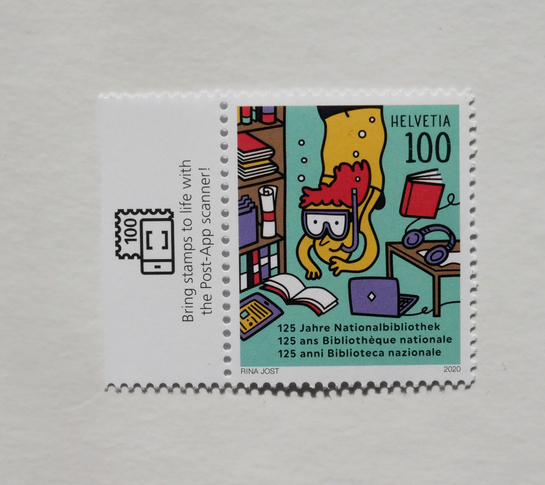
\includegraphics[width=0.6\textwidth]{img/schweiz-nationalbibliothek.jpg}
\caption{Briefmarke ``125 Jahre Nationalbibliothek'' aus der Schweiz}
\end{figure}

Pattriz. \emph{Puzzle ``Wimmelbild Bibliothek''} (2019)\\
Supportyourlocalartist.ch
(\url{https://supportyourlocalartists.bigcartel.com/}) ist ein während
der COVID-19-Krise aufgesetzter Shop, über den lokale (schweizerische)
Künstler*innen vor allem aus dem Schnittfeld Design und Street Art ihre
Werke anbieten. Sowohl Kunst als auch Preise sind sehr zugänglich. Nicht
nur kleine Verlage und Buchhandlungen, sondern selbstverständlich auch
so zugängliche Kunst sollte während der Krise unterstützt werden. Unter
anderem im Einkaufswagen landete das Puzzle ``Wimmelbild Bibliothek'',
welches die Illustratorin Pattriz letztes Jahr für das 5-jährige
Jubiläum der Stadtbibliothek Rapperswil-Jona im neuen Gebäude gestaltet
hatte. (\url{http://pattriz.ch/portfolio/stadtbibliothek/})

\begin{figure}[ht!]
\centering
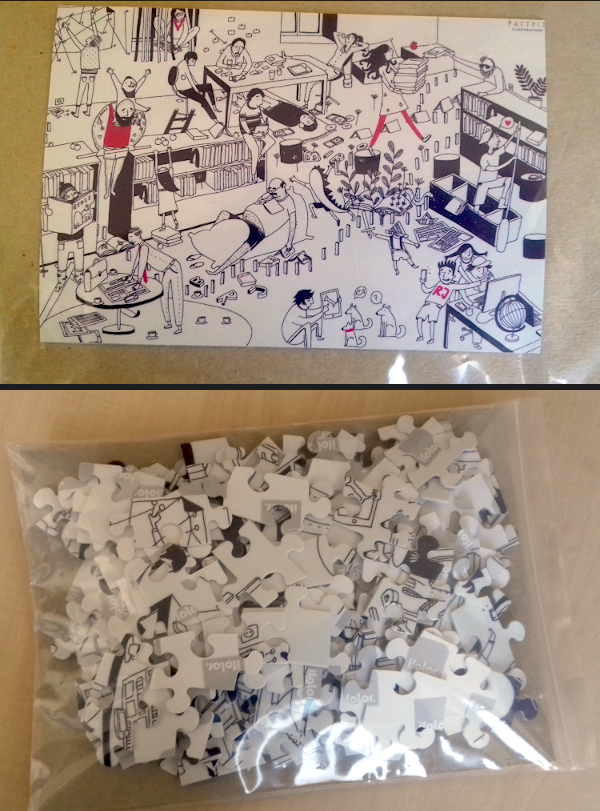
\includegraphics[width=0.8\textwidth]{img/puzzle-wimmelbild_bibliothek.jpg}
\caption{Puzzle ``Wimmelbild Bibliothek'' der Illustratorin Pattriz}
\end{figure}

Da aktuell nicht alle nach Rapperswil-Jona fahren können, um sich die
wirklich hellen Räume der Bibliothek live anzuschauen, sei dieses Puzzle
als unterhaltsamer Ersatz empfohlen. (ks)

%autor

\end{document}
